% easychair.tex,v 3.4 2016/10/19
\documentclass[EPiC]{easychair}

\usepackage{doc}
\usepackage{tikz}
\usepackage{subfigure}
\usepackage{tabularx}
\usepackage{booktabs}
\usepackage{framed}
\usepackage{amsmath,amssymb,amsfonts}
\usepackage{hyperref}
\usepackage[defaultlines=4,all]{nowidow}
\usepackage{enumitem} % GF 2017-03-28
\usepackage{tablefootnote}
\usepackage{cleveref}
\usepackage{xcolor}
\usepackage{floatrow}
\usepackage{tikz}
\usepackage{pbox}
\usepackage{pgfplots}

%% - Utils
\newlength{\plotwidth}
\setlength{\plotwidth}{0.45\columnwidth}
\newlength{\plotwidthShort}
\setlength{\plotwidthShort}{0.4\columnwidth}

% ---------------- Commands --------------------

\definecolor{lightblue}{RGB}{210,210,225}
\definecolor{lightred}{RGB}{235,220,220}
\definecolor{lightgreen}{RGB}{215,245,215}
\definecolor{lightyellow}{RGB}{225,222,200}
\definecolor{lightpurple}{RGB}{225,210,225}
\definecolor{darkblue}{RGB}{0,0,128}
\definecolor{darkred}{RGB}{128,0,0}
\definecolor{darkerred}{RGB}{64,0,0}
\definecolor{darkgreen}{RGB}{0,108,0}
\definecolor{darkyellow}{RGB}{25,22,0}
\definecolor{darkpurple}{RGB}{128,0,128}

\newcommand{\cyan}[1]{{\color{cyan}#1}}
\newcommand{\blue}[1]{{\color{blue}#1}}
\newcommand{\red}[1]{{\color{red}#1}}
\newcommand{\cmark}{\ding{51}}%
\newcommand{\xmark}{\ding{55}}%

% Abbreviated form for internal references (cleveref package)
\Crefname{section}{Sec.}{Secs.}
\crefname{section}{section}{sections}
\Crefname{subsection}{Sec.}{Secs.}
\crefname{subsection}{section}{sections}
\Crefname{equation}{Eq.}{Eqs.}
\crefname{equation}{eq.}{eqs.}
\Crefname{algorithm}{Alg.}{Algs.}
\crefname{algorithm}{algorithm}{algorithms}
\Crefname{table}{Tab.}{Tabs.}
\crefname{table}{table}{tables}
\Crefname{figure}{Fig.}{Figs.}
\crefname{figure}{figure}{figures}

% Make \paragraph{} bold font
\makeatletter
\renewcommand{\paragraph}{\@startsection{paragraph}{4}{0pt}%
  {.8ex plus 0.2ex minus 0.2ex}%
  {-0.5em}%
  {\bfseries}}
\makeatother

\newcommand{\dummyfig}[3]{\textcolor{Gray!30!#3!50}{\rule{#1}{#2}}}
\newcommand{\colorpar}[3]{\colorbox{#1}{\parbox{#2}{#3}}}
\newcommand{\marginremark}[4]{
  \marginpar{\colorpar{#2}{\linewidth}{\color{#1}\tiny{[#3] #4}}}}
\newcommand{\inlineremark}[4]{
  \par\noindent\colorpar{#2}{0.98\linewidth}{\color{#1}\tiny{[#3] #4}}\par}
\makeatletter
\def\THICKhrulefill{\leavevmode \leaders \hrule height 5pt\hfill \kern \z@}
\makeatother
\newcommand{\highlightedremark}[4]{%
  \begin{center}\fcolorbox{#1}{#2}{%
  \begin{minipage}{.98\linewidth}\color{#1}%
  \textbf{\THICKhrulefill[ #3 ]\THICKhrulefill}%
  \par\noindent#4\end{minipage}}\end{center}%
}

\newcommand{\TODO}[1]{\highlightedremark{darkred}{lightred}{TODO}{#1}}

% Remarks
\iftrue
  \newcommand{\rmkNMC}[1]{\marginremark{red}{red!25}{NMC}{#1}}
  \newcommand{\rmkAB}[1]{\marginremark{darkgreen}{Aquamarine!15}{AB}{#1}}
  \newcommand{\rmkAH}[1]{\marginremark{darkgreen}{Aquamarine!15}{AH}{#1}}
  \newcommand{\rmkVS}[1]{\marginremark{darkgreen}{Aquamarine!15}{VS}{#1}}
  \newcommand{\rmkHB}[1]{\marginremark{darkblue}{lightblue}{HB}{#1}}
  \newcommand{\rmkSS}[1]{\marginremark{darkbyellow}{lightyellow}{SS}{#1}}
  \newcommand{\rmkAA} [1]{\marginremark{darkpurple}{lightpurple}{AA}{#1}}
  \newcommand{\rmkSH} [1]{\marginremark{darkpurple}{lightpurple}{SH}{#1}}
  \newcommand{\rmkCV} [1]{\marginremark{darkpurple}{lightpurple}{CV}{#1}}
\else
  \newcommand{\rmkNMC}[1]{}
  \newcommand{\rmkAB}[1]{}
  \newcommand{\rmkAH}[1]{}
  \newcommand{\rmkVS}[1]{}
  \newcommand{\rmkHB}[1]{}
  \newcommand{\rmkSS}[1]{}
  \newcommand{\rmkAA}[1]{}
  \newcommand{\rmkSH}[1]{}
  \newcommand{\rmkCV}[1]{}
\fi

% Highlighted remarks
\newcommand{\hrmkNMC}[1]{\highlightedremark{darkred}{lightred}{NMC}{#1}}
\newcommand{\hrmkAB}[1]{\highlightedremark{darkgreen}{lightyellow}{AB}{#1}}
\newcommand{\hrmkAH}[1]{\highlightedremark{darkblue}{lightblue}{AH}{#1}}
\newcommand{\hrmkVS}[1]{\highlightedremark{darkbyellow}{lightyellow}{VS}{#1}}
\newcommand{\hrmkHB}[1]{\highlightedremark{darkbyellow}{lightyellow}{HB}{#1}}
\newcommand{\hrmkSS}[1]{\highlightedremark{darkbyellow}{lightyellow}{SS}{#1}}
\newcommand{\hrmkAA}[1] {\highlightedremark{darkpurple}{lightpurple}{AA}{#1}}
\newcommand{\hrmkSH}[1] {\highlightedremark{darkpurple}{lightpurple}{SH}{#1}}
\newcommand{\hrmkCV}[1]{\highlightedremark{darkbyellow}{lightyellow}{CV}{#1}}

\newcommand{\hey}[1]{\textbf{\color{Red}\sffamily\larger @{#1}:}\xspace}
\newcommand{\tocite}{%
  \marginremark{BrickRed}{white}{$\blacksquare$}{\textbf{citation~needed}\hfill}%
  \texttt{\color{Red}$\backslash$REF}\xspace}


\newcommand{\todo}[1]{
  \begin{framed}
    \noindent{\bf TODO: }
    #1
  \end{framed}
}
\newcommand{\remark}[1]{
  \begin{framed}
    \noindent{\bf Remark: }
    #1
  \end{framed}
}
%\makeindex

%% Front Matter
%%
% Regular title as in the article class.
%
\title{ARCH-COMP18 Category Report:\\ Stochastic Modelling}

% Authors are joined by \and. Their affiliations are given by \inst, which indexes
% into the list defined using \institute
% Author order: first author is group leader, other authors are added alphabetically
\author{Alessandro Abate \inst{1}
\and Henk Blom \inst{2}
\and Nathalie Cauchi \inst{1}
\and Sofie Haesaert \inst{3}
\and Arnd Hartmanns \inst{4}
\and Meeko Oisho \inst{5}
\and Soudjani Sadegh \inst{6}
\and  Vignesh Sivaramakrishnan  \inst{5}
\and  Cristian Vasile \inst{7}
 \and Abraham Vinod  \inst{5}
 }

% Institutes for affiliations are also joined by \and,
\institute{ University of Oxford,
Department of Computer Science,
Oxford, UK
  \email{name.surname@cs.ox.ac.uk}}

%  \authorrunning{} has to be set for the shorter version of the authors' names;
% otherwise a warning will be rendered in the running heads. When processed by
% EasyChair, this command is mandatory: a document without \authorrunning
% will be rejected by EasyChair

\authorrunning{}

% \titlerunning{} has to be set to either the main title or its shorter
% version for the running heads. When processed by
% EasyChair, this command is mandatory: a document without \titlerunning
% will be rejected by EasyChair
\titlerunning{ARCH-COMP18 Stochastic models}

\begin{document}

\maketitle
\todo{Add all affiliations}

\begin{abstract}
This report presents the results of a friendly competition for formal verification of continuous and hybrid systems with linear continuous dynamics. The friendly competition took place as part of the workshop \underline{A}pplied Ve\underline{r}ification for \underline{C}ontinuous and \underline{H}ybrid Systems (ARCH) in 2018. 
\end{abstract}

%------------------------------------------------------------------------------
\section{Introduction}
\label{sect:introduction}

\begin{framed}
\paragraph{Disclaimer} The presented report of the ARCH friendly competition for \textit{stochastic modelling group} which aims at providing a landscape ....
\end{framed}

This report summarizes results obtained in the 2018 friendly competition of the ARCH workshop\footnote{Workshop on \underline{A}pplied Ve\underline{r}ification for \underline{C}ontinuous and \underline{H}ybrid Systems (ARCH), \href{http://cps-vo.org/group/ARCH}{cps-vo.org/group/ARCH}} for\\ 
 
 

The goal of the friendly competition is not to rank the results, but rather to present the landscape of existing solutions in a breadth that is not possible with scientific publications in classical venues. Such publications would typically require the presentation of novel techniques, while this report showcases the current state-of-the-art tools. For all results reported by each participant, we have run an independent repeatability evaluation. 

\hrmkNMC{To complete}

%------------------------------------------------------------------------------
\section{Benchmarks}
\label{sec:benchmarks}

We introduce a new category for the 2018 edition and with it a new set of benchmarks: an anesthesia delivery system, building automation system, a heated tank, a lawn mover and a mars rover. Each benchmark is characterised with special features which we delineate first. Next, we discuss each benchmark, the different problems to be solved together with specifications of interest, and different paths to successfully verifying a benchmark. Afterwards, the verification of each benchmark is presented in detail. \\

\paragraph{Special features} We briefly list the key features of each benchmark:
\begin{itemize}
	\item \textit{Anesthesia delivery system benchmark}: 
	\item \textit{Building automation benchmark}: this benchmark is based on a library of models describing different components within a heating system. We focus on two instances of possible benchmarks which describe discrete-time linear systems with varying numbers of continuous state variables. The benchmark focuses on safety properties.
	\item \textit{Heated tank benchmark}: 
    \item \textit{Lawn mower benchmark}:
    \item \textit{Mars rover benchmark}:
\end{itemize}

\todo{Include brief description or special features of the benchmark}

%%% Benchmark descriptions together with results
\subsection{Anesthesia Delivery System Benchmark}
\newpage

\subsection{Building Automation System Benchmark}
The Building Automation System (BAS) benchmark is a modular and extendable benchmark  constructed from a library of stochastic models representing the different components making up a BAS. The library of models is presented in~\cite{Cauchi18ADHS} and the reader is referred to the afore-cited paper for more details. Using this
library of models we setup two instances which aim to address  verification and policy synthesis respectively. We denote the first instance as CS1BAS, while the second instance as CS2BAS.
For each (i) we establish the dynamics of the models, (ii) the specification of interest, and (iii) we describe possible solutions.
he model is available in Matlab format on the ARCH website \rmkNMC{add url}.

\subsubsection{CS1BAS: Model} 
\begin{figure}[h!]
    \centering
 	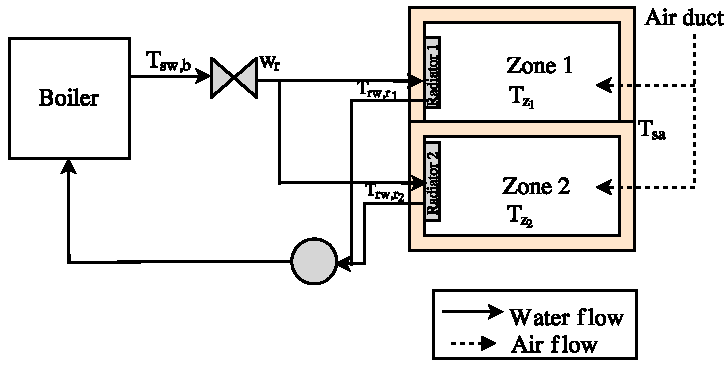
\includegraphics[width=0.5\columnwidth]{figures/Cs1.pdf}
 	\caption{figure}{BAS setup for the first case study}
 	\label{fig:cs1:setup}
 \end{figure}
 
We consider two zones, each heated by one radiator and with a common supply air, as portrayed in Figure~\ref{fig:cs1:setup}. 
The model is described as stochastic linear discrete-time model
\begin{equation}\label{mod:s}
	\textbf{M}_s: \begin{cases}
	x[k+1] &=Ax[k] + Bu[k] + Q + \Sigma W[k] \\ % \in \Rl^4 \\
	y_s[k] &= \begin{bmatrix}
	1&0&0&0\\
	0&1&0&0\end{bmatrix} x[k], 
	\end{cases}
\end{equation}
with a uniform sampling time $\Delta=$ 15 minutes. Here, the matrices $A, \; B, \; Q $ are properly sized  and \resizebox{0.55\textwidth}{!}{$ \Sigma = diag([(\sqrt{\Delta}\sigma_{z_1})^2 \; (\sqrt{\Delta}\sigma_{z_2})^2 \;(\sqrt{\Delta}\sigma_{rw,r_1})^2 \;(\sqrt{\Delta}\sigma_{rw,r_2})^2])$}
encompasses the variances of the process noise for each state. $W = \begin{bmatrix}w_1& w_2& w_3& w_4\end{bmatrix}^T$ are independent Gaussian random variables, which are also independent of the initial condition of the process. The exact matrix values are kept within the ARCH repository.

\subsubsection{CS1BAS: Specifications}
We consider the stochastic safety property:  to decide whether traces generated by the models remain within a specified safe set for a given time period. Specifically, this is described using the PCTL property:
\begin{equation*}
\Phi:= \mathbb{P}_{= p} [\square^{\le N=1.5\text{hours}}\; \mathcal{S}]
\end{equation*}
where $p$ is the probability of satisfaction, $\mathcal{S}$ is the safe set is described as an interval around the temperature set-point $T_{SP} = 20^oC$ $\pm 0.5^oC$, specifically, 
\begin{align*}
\mathcal{S}&=\begin{bmatrix}
19.5 & 20.5 \\
19.5 & 20.5 \\
19.5 & 20.5 \\
19.5 & 20.5 \\
\end{bmatrix}.
\end{align*}
We defined the acceptable probability of the specification to be true for $p \ge 0.9$.

\subsubsection{CS2BAS: Model} 
In this second case study we focus on the {stochastic} dynamics of the zone component. The model is a discrete-time model with a sampling time $\Delta = 15$ minutes, and takes the form of
\begin{equation}
	\textbf{M}_{c}:
	\begin{cases}
	x_c[k+1] &= 
	A_{c}x_c[k] +B_cu_c[k]	+ F_{c}d_c[k]+ Q_c\\
	y_c[k]   &= \begin{bmatrix}
	1&0&0&0&0&0&0 \end{bmatrix}x_c[k]. 
	\end{cases}%$}
	\label{eqn:Mc}
\end{equation}
Here the continuous state variable $x_c$ is composed of 7 states representing the zone and wall temperatures, the input $u_c$ corresponds of the fan supply rate having a dimension of 1. The disturbance vector $d_c$ has a dimension of 6 which represent external heat sources (weather, occupancy, radiators), while $Q_c$ represents constant additive terms within the model. We model the disturbances as random external effects following  Gaussian distributions with a mean $\mu$ and variance $\sigma$,  affecting the room temperature dynamics as $T_{out}[k] \sim  \mathcal{N}(\mu=9,\sigma=1),~T_{hall}[k] \sim \mathcal{N}(\mu=15,\sigma=1),\; CO_{2_i}[k] \sim  \mathcal{N}(\mu=500,\sigma=100), i \in \{1,2\},\;
T_{rw,r_i}[k] \sim  \mathcal{N} (\mu =35, \sigma=5), i \in \{1,2\}$.\\

\subsubsection{CS2BAS: Specifications}
We would like to synthesise a policy ensuring that the temperature within zone 1 does not deviate from the set point by more then 0.5$^oC$ over a time horizon equal to four hours (i.e $N= 16$). This can be translated into following PCTL specification:
\begin{equation*}
\Phi:= \mathbb{P}_{= p} [\square^{\le N=16} \; |T_{z_1}-T_{SP}| \le 0.5]
\end{equation*}
over which $p$ is to be maximised for the optimal policy. Here, $T_{SP} = 20^oC$.


\newpage

\subsection{Heated Tank Benchmark}
\newpage

\subsection{Lawn Mower Benchmark}
Here we describe dynamics of a lawn mower as introduced in \cite{foldager2017development}. A conceptual model of the driverless lawn mower is shown in Fig. \ref{subfig1}. The lawn mower is steered by controlling the velocity separately on the two driving wheels. A sketch of the vehicle is shown in Fig. \ref{subfig2} and its chassis and caster wheels are shown in Fig. \ref{subfig3}.
\begin{figure}[hpt]
\centering
\subfigure[]{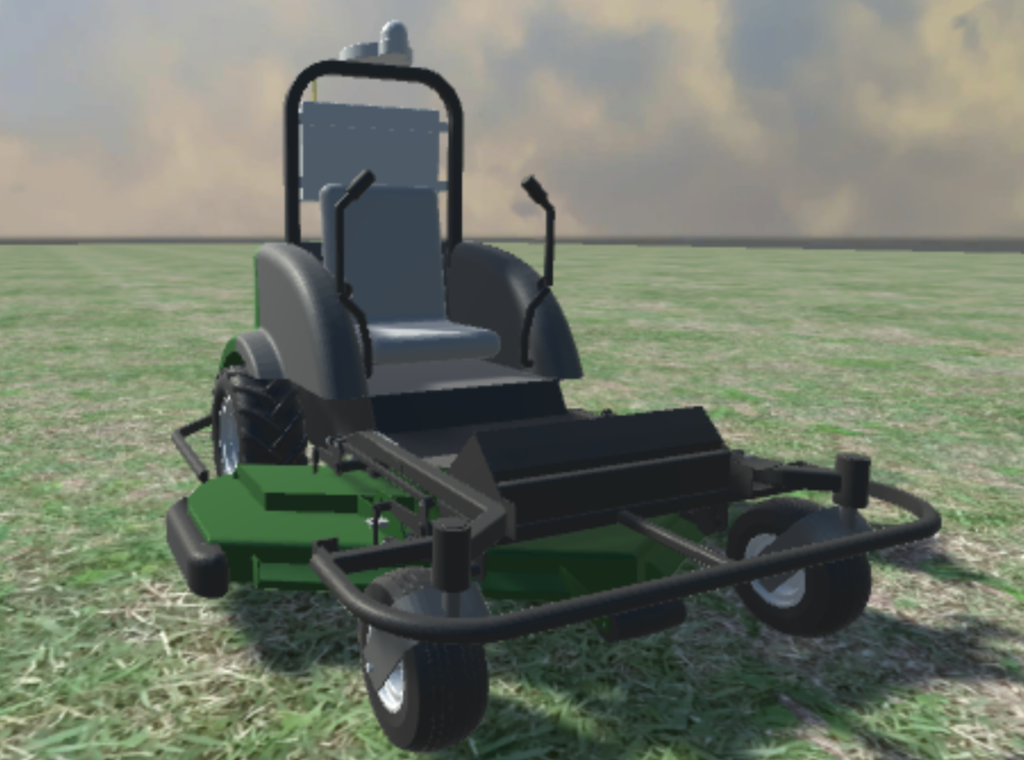
\includegraphics[scale=0.26]{figures/Lawn_Mower.png}\label{subfig1}}
\subfigure[]{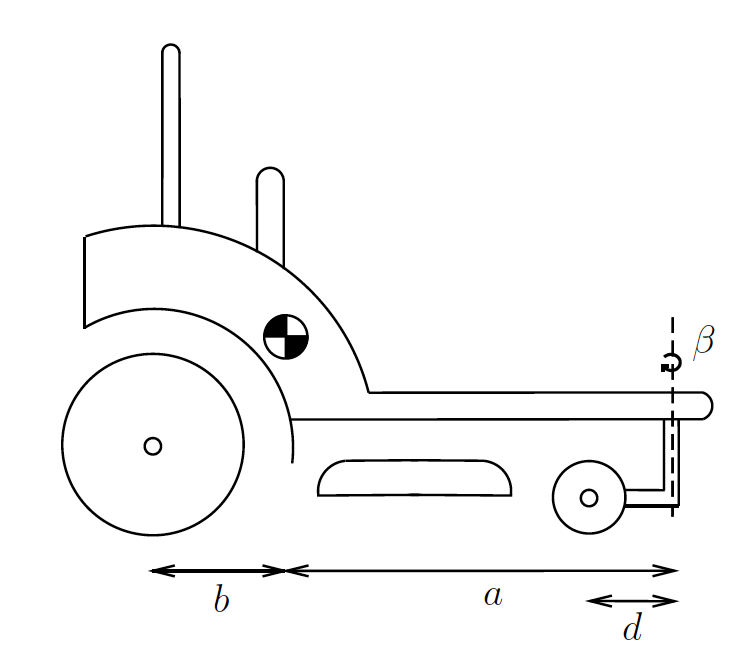
\includegraphics[scale=0.19]{figures/fig1.png}\label{subfig2}}
\subfigure[]{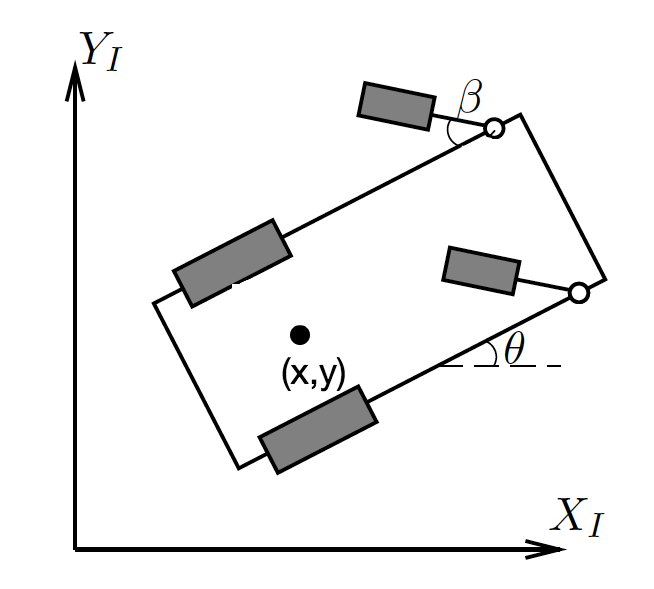
\includegraphics[scale=0.19]{figures/fig2_1.png}\label{subfig3}}
\caption{Lawn mower schematics \cite{foldager2017development}}
\label{Lawn_Mower}
\end{figure}

\subsubsection{Dynamical model}
The dynamic response of the lawn mower can be described by the following 6-dimensional nonlinear stochastic differential equation
\begin{align}
\dot{x}_1 &= \frac{1}{I_{zz}}\left ( A_{fy}\sin\Big ( x_6+\frac{\pi}{2}\Big )a+2C_{\gamma}\tan\Big ( \frac{2(x_2-bx_1)}{(V_r+V_l)}\Big )b \right ),\nonumber\\
\dot{x}_2 &= \frac{1}{M}\left ( A_{fy}\sin\Big ( x_6+\frac{\pi}{2}\Big )-2C_{\gamma}\tan\Big(  \frac{2(x_2-bx_1)}{(V_r+V_l)}\Big )\right )- \frac{V_r+V_l}{2}x_1,\nonumber\\
\dot{x}_3 &= \frac{V_r+V_l}{2}\cos(x_5),\\
\dot{x}_4 &= \frac{V_r+V_l}{2}\sin(x_5),\nonumber\\
\dot{x}_5 &= \frac{V_r-V_l}{2D}+x_1+w_{d1},\nonumber\\
\dot{x}_6 &= -\frac{V_r+V_l}{2d}\cos(x_6)-\frac{(V_r-V_l)(d+\sqrt{D^2+(a+b)^2}\sin(x_6))}{2Dd}+w_{d2},\nonumber
\end{align}
where $x_1$, $x_2$, $x_3$, $x_4$, $x_5$, and $x_6$ are respectively yaw, yaw rate, $x$, $y$, angle of vehicle with respect to $x$-axis ($\theta$), and relative orientation of caster wheel ($\beta$), respectively. The $w_{d1}$ and $w_{d2}$ are noises in orientation and angle of caster wheel generated due to uneven ground surface. $V_r$ and $V_l$ are the control inputs representing velocity of right and left driving wheels, respectively.
%Fig.~\ref{Lawn_Mower} shows the schematic of lawn mower.
The remaining parameters are listed in Table~\ref{table_parameter}.
% Please add the following required packages to your document preamble:
% \usepackage{booktabs}
\begin{table}[]
\centering
\caption{Lawn mower parameters}
\label{table_parameter}
\begin{tabular}{@{}ll@{}}
\toprule
Mass, M                      & 700$kg$                     \\
Axle half width, D                & 1.2$m$                      \\
Dimensions, (a, b)           & 1.35$m$, 0.15$m$                \\
Caster wheel offset, d       & 0.1$m$                        \\
$A_{fy}$                    & 199                         \\
$I_{zz}$                    & 394 $Kg$-$m^2$ \\
$C_{\gamma}$ & 22000                       \\ \bottomrule
\end{tabular}
\end{table}

It is possible to extend the dynamics by modelling the response of the steering mechanism using a first order equation for each driving wheel:
\begin{align*}
\dot{V_l} = -k_\tau\cdot (V_l - V_l^{sp}),\\
\dot{V_r} = -k_\tau\cdot (V_r - V_r^{sp}),
\end{align*}
where $V_l^{sp}$ and $V_r^{sp}$ are velocity set points specified by the controller, and $k_\tau$ is a gain determined experimentally.
In the following, we assume that velocities $V_l$ and $V_r$ can be directly specified by the controller. In other words, $k_\tau$ is very large in compare with the sampling time of the controller and $V_l(t)\approx V_l^{sp}$ and $V_r(t) \approx V_r^{sp}$.

\subsubsection{Controller mechanism}
The main objective for the lawn mower is to cover a given area as soon as it can. This can be seen as a path planning problem and is usually achieved by specifying a set of way-points, and the task of the controller would be to move from an initial position in the vicinity of the current way-point to the vicinity of the next way-point.
%\noindent
%\textbf{Controller 1.}
We provide simple On-Off type controller for lawn mover to reach desired position $(x_d,y_d)$. Consider base velocity $V_b$ and boost velocity $V_d$.  
 The control inputs that is velocities of right and left wheel are given as
\begin{align}
V_r&=V_b+V_d \text{sgn}(\sin(\theta_d-x_5))\nonumber\\
V_l&=V_b-V_d \text{sgn}(\sin(\theta_d-x_5)),\label{eq:controller}
\end{align}
where $\theta_d=\text{atan2}((y_d-x_4),(x_d-x_3))$.
The closed-loop response starting from initial condition $[0,0,0,0,0]^T$ reaching desired location $(x_d,y_d)=(-10,-5)$ with selection of $V_b=2$ and $V_d=1.5$ is shown in Fig.~\ref{fig3}.
\begin{figure}[hpt]
\centering
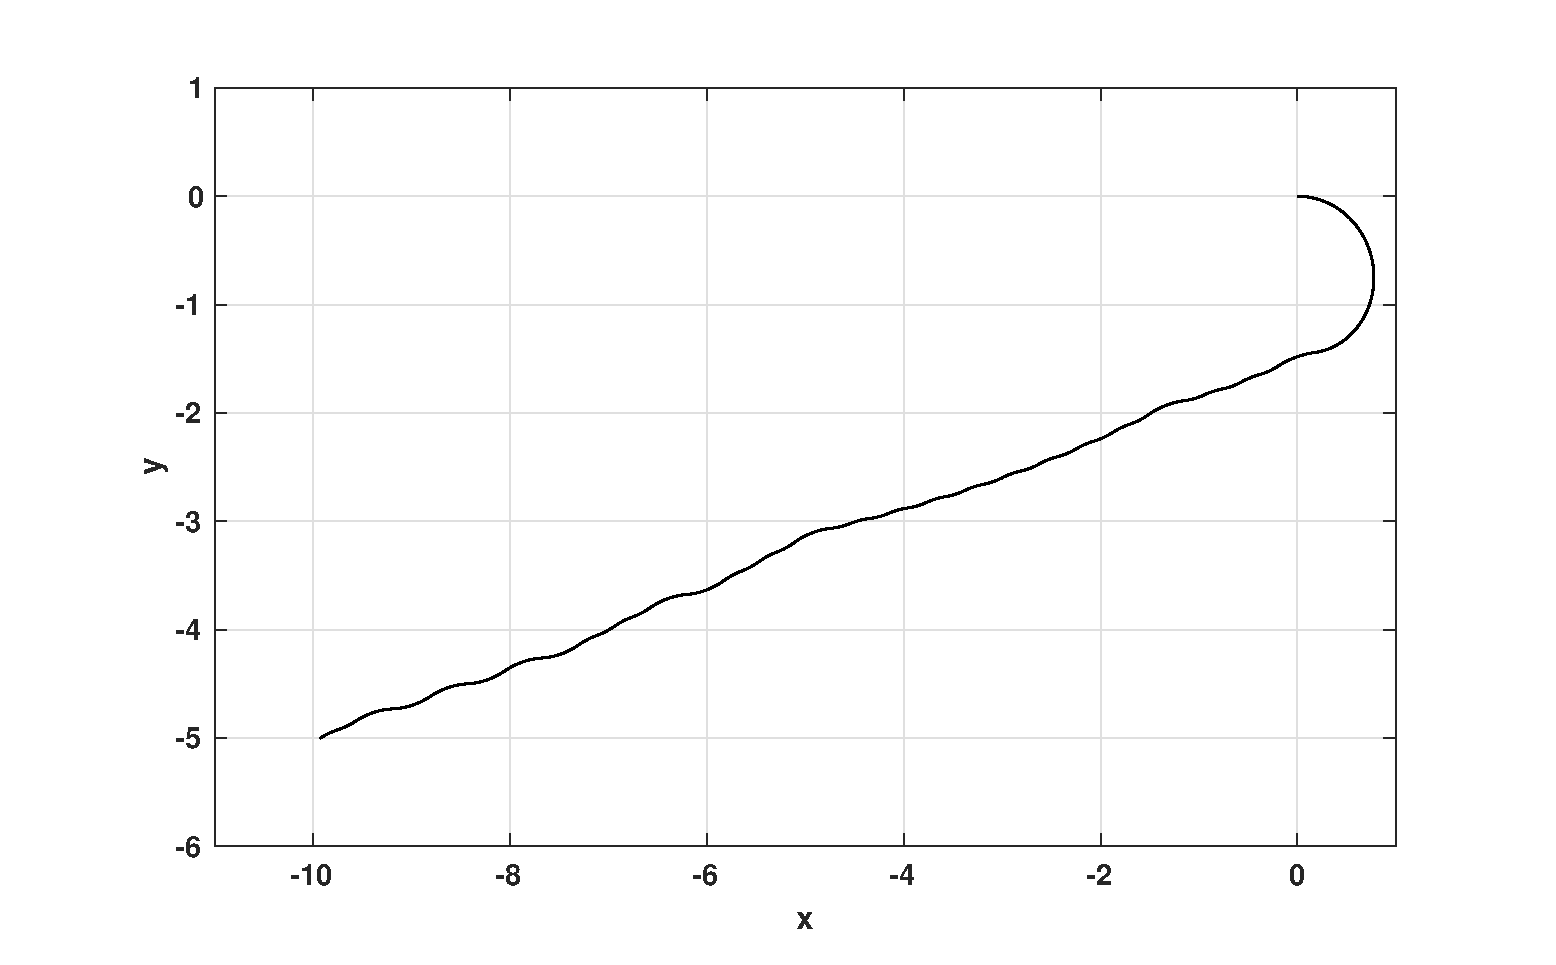
\includegraphics[scale=0.8,height=5cm]{figures/resp1}
\caption{Closed-loop response of lawn mower}
\label{fig3}
\end{figure}

% \noindent
% \textbf{Controller 2.}
% We provide PI controller for lawn mover to reach desired position $(x_d,y_d)$. Consider base velocity $V_b$, and $u_1$ and $u_2$ as a boost velocity for right and left wheels, respectively. The velocity of right and left wheel is given as
% \begin{align*}
% V_r&=V_b+u_1,\\
% V_l&=V_b+u_2.
% \end{align*}
% The error in current position and desired position is given by $e_p=\sqrt{(x_d-x_3)^2+(y_d-x_4)^2}$ and is used to calculate base velocity as $V_b=k_p e_p$, where $k_p>0$ is a proportional gain. For computing $u_1$ and 
% $u_2$, we need misalignment between the orientation of vehicle and orientation of desired position, and it is calculated as
% \[\theta_e=\text{atan2}(\sin(\theta_d-x_5),\cos(\theta_d-x_5)),\]
% where $\theta_d=\text{atan2}((y_d-x_4),(x_d-x_3))$. The $u_1$ and $u_2$ are computed as
% \begin{align*}
% \begin{matrix}
% \begin{bmatrix}
% u_1\\ 
% u_2
% \end{bmatrix}=\begin{bmatrix}k\theta_e+k_i\int \theta_e\\ 
% 0
% \end{bmatrix}, & \text{if } \theta_e>0,
% \\
% \begin{bmatrix}
% u_1\\ 
% u_2
% \end{bmatrix}=\begin{bmatrix}0\\ 
% k\theta_e+k_i\int \theta_e
% \end{bmatrix}, & \text{if } \theta_e<0,
% \end{matrix}
% \end{align*}  
% where $k,k_i>0$ are proportional and integral gains. The trajectory starting from initial condition $[0,0,0,0,0]^T$ reaching desired location $(x_d,y_d)=(-10,-5)$ is shown in Figure \ref{fig2}.
% \begin{figure}[hpt]
% \centering
% 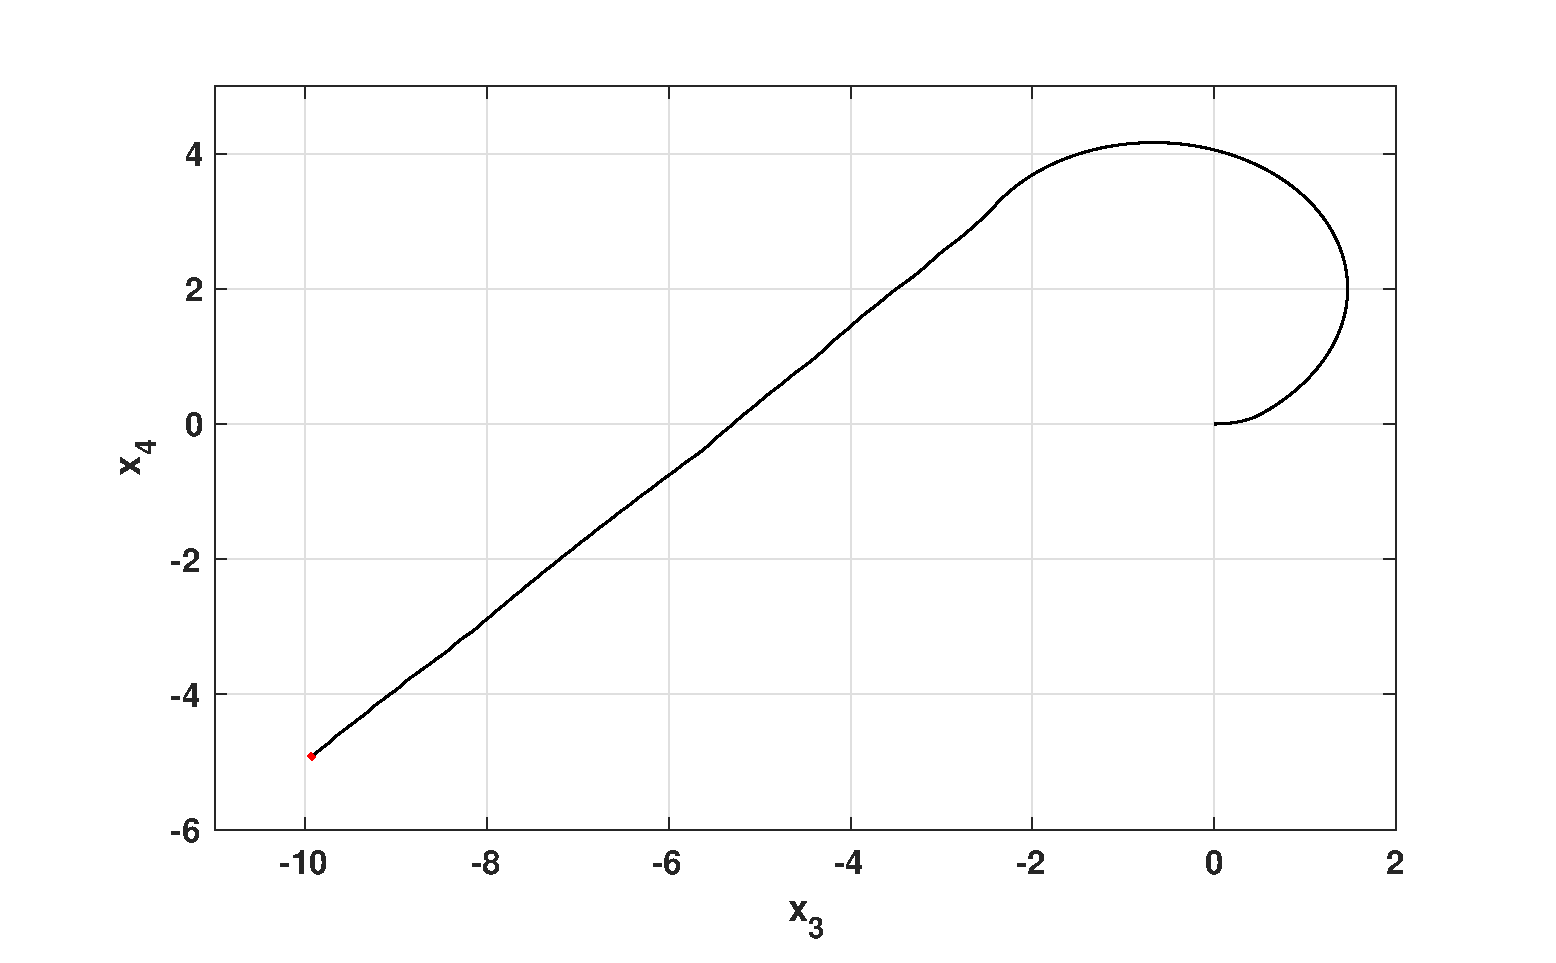
\includegraphics[scale=0.8,height=5cm]{figures/resp}
% \caption{Closed-loop response of lawn mower}
% \label{fig2}
% \end{figure} 

\subsubsection{Specification of interest}
% Therefore, the first interesting problem will be to find probability of reaching a target set while avoiding hitting boundaries of the area.
%\begin{equation*}
%\mathbb P()
%\end{equation*}
The controller of the previous subsection does not take into account avoiding obstacles and preventing collision with boundaries of the area. Here we define a specification that computes probability of avoiding obstacles over finite-time traces of the system. 

The state space of the system is $X=\mathbb R^{6}$. We consider the region $X_0 = [-0.5,0.5]^2\times[-1,1]^2\times[-\pi,\pi]^2$ for the initial state of the system and $X_1 = [-0.5,0.5]^2\times[-4,4]\times[2.5,4]\times[-\pi,\pi]^2$ for the obstacles or one of the boundaries of the area. The set of atomic propositions is given by $\Pi=\{p_0,p_1,p_2\}$ with labeling function $L(x_i) = p_i$ for all $x_i\in X_i$, $i\in\{0,1,2\}$, with $X_2 := X\backslash (X_0\cup X_1)$ . The objective is to compute a lower bound $\alpha>0$ on the probability that the solution process of length $N=200$ satisfies the safe LTL$_f$ formula $p_0\wedge\square^{\le 200}\neg p_1$:
$$\Phi:=\mathbb P_{\ge \alpha}[p_0\wedge\square^{\le 200}\neg p_1].$$

% The next rather complicated problem would be to design a control strategy for fully covering the area using a set of way-points and then ask for the probability of full covering as a function of time.
% Here we tackle the reachability problem.

%\subsection{Reachability Probability}


\newpage

\subsection{Mars Rover Benchmark}

\todo{Inclusion of full benchmark descriptions and results of case-studies}

%------------------------------------------------------------------------------
\section{Participating Tools}
\label{sect:tools}

The tools  participating in the category \textit{Stochastic Modelling} are introduced subsequently in alphabetical order.


\paragraph{FAUST$^2$}
The tool \textit{Formal Abstractions of Uncountable-STate STochastic
processes} (FAUST$^2$) ~\cite{soudjani2015faust} generates formal abstractions of discrete-time Markov processes (dtMP) defined over continuous state spaces. The dtMP model is abstracted into a finite-state Markov chain or a Markov decision process. The abstract model is formally put in relationship with the concrete dtMP via a user-defined maximum threshold on the approximation error introduced by the abstraction procedure. FAUST 2 allows exporting the abstract model to well-known probabilistic model checkers,such as PRISM or MRMC. Alternatively, it can handle internally the com-
putation of PCTL properties (e.g. safety or reach-avoid) over the abstract model, and refine the outcomes over the concrete dtMP via a quantified error that depends on the abstraction procedure and the given formula. The toolbox is available at \url{https://sourceforge.net/projects/faust2/}\\

\paragraph{Modest}

\paragraph{SReach Tools}


\todo{ Fill the appropriate description + title of tool or framework employed}
%------------------------------------------------------------------------------
\section{Results}
\label{sect:results}

We present the results obtained for each case studies using the tools highlighted in Sec.\ref{sect:tools}.

%%%%% Results for Anesthesia model
\subsection{Anesthesia benchmark}
\newpage

\subsection{Building Automation System benchmark}
\subsubsection{CS1BAS: Results}
The results obtained using the individual tools are presented hereunder. 
\begin{figure}[htb]
\centering
\resizebox{0.6\columnwidth}{!}{% This file was created by matlab2tikz.
%
%The latest updates can be retrieved from
%  http://www.mathworks.com/matlabcentral/fileexchange/22022-matlab2tikz-matlab2tikz
%where you can also make suggestions and rate matlab2tikz.
%
\begin{tikzpicture}
\begin{axis}[%
width=2.5in,
height=1.3in,
at={(0,0)},
scale only axis,
point meta min=0.470282235842186,
point meta max=0.986564815040043,
colormap/jet,
xmin=19.5,
xmax=20.5,
xlabel={$T_{z_1} (^oC)$},
xtick={19.5, 20, 20.5},
ytick={19.5, 20, 20.5},
ymin=19.5,
ymax=20.5,
ylabel={$T_{z_2}(^oC)$},
axis background/.style={fill=white},
axis x line*=bottom,
axis y line*=left,
xmajorgrids,
ymajorgrids,
colorbar
]

\addplot[area legend, table/row sep=crcr, patch, patch type=rectangle, draw opacity=0, shader=flat corner, draw=black, forget plot, patch table with point meta={%
0	1	2	3	0.827893902775227\\
4	5	6	7	0.793024086765995\\
8	9	10	11	0.746564890317088\\
12	13	14	15	0.681456944665337\\
16	17	18	19	0.590236031136011\\
20	21	22	23	0.470282235842186\\
24	25	26	27	0.791550953578066\\
28	29	30	31	0.743800828154144\\
32	33	34	35	0.677722355606167\\
36	37	38	39	0.572868018218282\\
40	41	42	43	0.824282040483261\\
44	45	46	47	0.784360583119843\\
48	49	50	51	0.721372278958824\\
52	53	54	55	0.614977823218979\\
56	57	58	59	0.808758487176058\\
60	61	62	63	0.746803206134085\\
64	65	66	67	0.638808800025938\\
68	69	70	71	0.861869517676606\\
72	73	74	75	0.825226177203703\\
76	77	78	79	0.763534677401247\\
80	81	82	83	0.65420762967246\\
84	85	86	87	0.837027060409398\\
88	89	90	91	0.775274305611174\\
92	93	94	95	0.664837996166706\\
96	97	98	99	0.845778949646682\\
100	101	102	103	0.783866801662126\\
104	105	106	107	0.672534150082666\\
108	109	110	111	0.887712727784528\\
112	113	114	115	0.851998575614929\\
116	117	118	119	0.790020997155602\\
120	121	122	123	0.678102271501412\\
124	125	126	127	0.856656414953906\\
128	129	130	131	0.794595367177973\\
132	133	134	135	0.682212778023659\\
136	137	138	139	0.860315889893475\\
140	141	142	143	0.798117094736825\\
144	145	146	147	0.685312687403086\\
148	149	150	151	0.898599310829689\\
152	153	154	155	0.863097520768723\\
156	157	158	159	0.800750295764352\\
160	161	162	163	0.687593331774096\\
164	165	166	167	0.864891564885841\\
168	169	170	171	0.802519215629093\\
172	173	174	175	0.689197663898604\\
176	177	178	179	0.901682384931356\\
180	181	182	183	0.866137430072826\\
184	185	186	187	0.803780890928022\\
188	189	190	191	0.690373054640137\\
192	193	194	195	0.945852328264193\\
196	197	198	199	0.941615919692457\\
200	201	202	203	0.937035477559722\\
204	205	206	207	0.932076256780272\\
208	209	210	211	0.926695817201953\\
212	213	214	215	0.920841960023429\\
216	217	218	219	0.914452141729648\\
220	221	222	223	0.907455486149551\\
224	225	226	227	0.899826205602794\\
228	229	230	231	0.891467063522451\\
232	233	234	235	0.882277022431808\\
236	237	238	239	0.872256161999317\\
240	241	242	243	0.861205390847799\\
244	245	246	247	0.848945927637339\\
248	249	250	251	0.953204580418968\\
252	253	254	255	0.949550500743908\\
256	257	258	259	0.945603192201279\\
260	261	262	263	0.941335745444352\\
264	265	266	267	0.936716010525619\\
268	269	270	271	0.931710875991253\\
272	273	274	275	0.926290302947337\\
276	277	278	279	0.920387074941379\\
280	281	282	283	0.913936785202574\\
284	285	286	287	0.906911970726105\\
288	289	290	291	0.899222391939057\\
292	293	294	295	0.890793062568912\\
296	297	298	299	0.88159083646468\\
300	301	302	303	0.871462506230663\\
304	305	306	307	0.860275488809037\\
308	309	310	311	0.847956804534903\\
312	313	314	315	0.834289364820515\\
316	317	318	319	0.818831091632674\\
320	321	322	323	0.95949763614734\\
324	325	326	327	0.956345059158354\\
328	329	330	331	0.952939954948432\\
332	333	334	335	0.949262019222174\\
336	337	338	339	0.945287969990615\\
340	341	342	343	0.940995653251133\\
344	345	346	347	0.936356763954177\\
348	349	350	351	0.931328545783152\\
352	353	354	355	0.925864429721092\\
356	357	358	359	0.919907738188407\\
360	361	362	363	0.913437263908993\\
364	365	366	367	0.906357841436535\\
368	369	370	371	0.898607016868959\\
372	373	374	375	0.89014745417327\\
376	377	378	379	0.880847524665068\\
380	381	382	383	0.870603085795288\\
384	385	386	387	0.859265235331487\\
388	389	390	391	0.846603440041587\\
392	393	394	395	0.964969890852782\\
396	397	398	399	0.962228216274421\\
400	401	402	403	0.959268691450228\\
404	405	406	407	0.956096339915495\\
408	409	410	411	0.95266837874538\\
412	413	414	415	0.948965353339708\\
416	417	418	419	0.944962888934275\\
420	421	422	423	0.94063192087226\\
424	425	426	427	0.93593740944021\\
428	429	430	431	0.930836337448006\\
432	433	434	435	0.925276040878729\\
436	437	438	439	0.919193949374637\\
440	441	442	443	0.91251891911906\\
444	445	446	447	0.905172102540523\\
448	449	450	451	0.89706294148596\\
452	453	454	455	0.888075745982356\\
456	457	458	459	0.878044928546052\\
460	461	462	463	0.866718545531803\\
464	465	466	467	0.853704682883987\\
468	469	470	471	0.838383629588774\\
472	473	474	475	0.969643917367778\\
476	477	478	479	0.967312574327892\\
480	481	482	483	0.964769675663228\\
484	485	486	487	0.962004213032771\\
488	489	490	491	0.959010206773037\\
492	493	494	495	0.955769783191322\\
496	497	498	499	0.952259752615276\\
500	501	502	503	0.948452696882103\\
504	505	506	507	0.944316080828982\\
508	509	510	511	0.939810436817739\\
512	513	514	515	0.934887002684482\\
516	517	518	519	0.92948522117762\\
520	521	522	523	0.923530347610091\\
524	525	526	527	0.916930835192949\\
528	529	530	531	0.909574345314996\\
532	533	534	535	0.901320101905455\\
536	537	538	539	0.891983643352544\\
540	541	542	543	0.881306958386857\\
544	545	546	547	0.973593955009027\\
548	549	550	551	0.97158104433421\\
552	553	554	555	0.969334955182894\\
556	557	558	559	0.966884182337719\\
560	561	562	563	0.964223059659987\\
564	565	566	567	0.961333715528205\\
568	569	570	571	0.958192596145299\\
572	573	574	575	0.954771527274864\\
576	577	578	579	0.951036804232258\\
580	581	582	583	0.946947373626039\\
584	585	586	587	0.942452560282376\\
588	589	590	591	0.937489732985685\\
592	593	594	595	0.931982094772026\\
596	597	598	599	0.925836101812086\\
600	601	602	603	0.918937023991266\\
604	605	606	607	0.911140209632807\\
608	609	610	611	0.902254372940749\\
612	613	614	615	0.892010495020195\\
616	617	618	619	0.880004277838634\\
620	621	622	623	0.865593755705279\\
624	625	626	627	0.976921636990858\\
628	629	630	631	0.975126380372231\\
632	633	634	635	0.973109188294971\\
636	637	638	639	0.970898811103174\\
640	641	642	643	0.968489593482401\\
644	645	646	647	0.96586336324951\\
648	649	650	651	0.962995834973554\\
652	653	654	655	0.959857513284957\\
656	657	658	659	0.956412627730787\\
660	661	662	663	0.952617288082819\\
664	665	666	667	0.948417549310501\\
668	669	670	671	0.943748014039979\\
672	673	674	675	0.938531047867573\\
676	677	678	679	0.932675296558365\\
680	681	682	683	0.926070653972229\\
684	685	686	687	0.918576326012426\\
688	689	690	691	0.909999256015899\\
692	693	694	695	0.900059327365279\\
696	697	698	699	0.888332119747655\\
700	701	702	703	0.874150707314913\\
704	705	706	707	0.97962017533361\\
708	709	710	711	0.977989950015278\\
712	713	714	715	0.976144420310686\\
716	717	718	719	0.974112278127227\\
720	721	722	723	0.971887726227782\\
724	725	726	727	0.969452428234577\\
728	729	730	731	0.966782018456432\\
732	733	734	735	0.963847196065247\\
736	737	738	739	0.960612906797647\\
740	741	742	743	0.957036592583544\\
744	745	746	747	0.953065743330998\\
748	749	750	751	0.948634899238956\\
752	753	754	755	0.943662294991566\\
756	757	758	759	0.938046224430796\\
760	761	762	763	0.931660708892112\\
764	765	766	767	0.924348748937713\\
768	769	770	771	0.915908759558779\\
772	773	774	775	0.906065328381823\\
776	777	778	779	0.981763993108222\\
780	781	782	783	0.980257177604919\\
784	785	786	787	0.978538904612199\\
788	789	790	791	0.976637674618032\\
792	793	794	795	0.974547475257295\\
796	797	798	799	0.972249806415611\\
800	801	802	803	0.969720266425377\\
804	805	806	807	0.966929768138499\\
808	809	810	811	0.963843861730206\\
812	813	814	815	0.960420995978192\\
816	817	818	819	0.956609711461877\\
820	821	822	823	0.952344638313184\\
824	825	826	827	0.947541548552388\\
828	829	830	831	0.942092395884218\\
832	833	834	835	0.935861370784495\\
836	837	838	839	0.92868118545443\\
840	841	842	843	0.920344242008159\\
844	845	846	847	0.910576719452606\\
848	849	850	851	0.898977827753047\\
852	853	854	855	0.884904741633888\\
856	857	858	859	0.983469730744431\\
860	861	862	863	0.982056712089993\\
864	865	866	867	0.980434925526348\\
868	869	870	871	0.978632701167642\\
872	873	874	875	0.976643786527943\\
876	877	878	879	0.974449359017563\\
880	881	882	883	0.972024568045206\\
884	885	886	887	0.969339646944809\\
888	889	890	891	0.966359096187905\\
892	893	894	895	0.963039889739201\\
896	897	898	899	0.959328892786201\\
900	901	902	903	0.955159588792252\\
904	905	906	907	0.950448319125091\\
908	909	910	911	0.945090264624252\\
912	913	914	915	0.938955015366494\\
916	917	918	919	0.931880190733888\\
920	921	922	923	0.923658542894369\\
924	925	926	927	0.91400913882808\\
928	929	930	931	0.902517320432239\\
932	933	934	935	0.888524052534189\\
936	937	938	939	0.98479623520115\\
940	941	942	943	0.983454202782001\\
944	945	946	947	0.981905901002911\\
948	949	950	951	0.980179605557133\\
952	953	954	955	0.978268841255738\\
956	957	958	959	0.976154310400871\\
960	961	962	963	0.973810285596792\\
964	965	966	967	0.971205499175553\\
968	969	970	971	0.968302084231217\\
972	973	974	975	0.965053741390793\\
976	977	978	979	0.961403764607638\\
980	981	982	983	0.957283478623712\\
984	985	986	987	0.952611125384509\\
988	989	990	991	0.947289979260307\\
992	993	994	995	0.941203053125515\\
996	997	998	999	0.934201213259913\\
1000	1001	1002	1003	0.926081841783896\\
1004	1005	1006	1007	0.916553923491709\\
1008	1009	1010	1011	0.985799987001766\\
1012	1013	1014	1015	0.984509581176649\\
1016	1017	1018	1019	0.983014777071847\\
1020	1021	1022	1023	0.981343860910171\\
1024	1025	1026	1027	0.979490250786347\\
1028	1029	1030	1031	0.977434414911\\
1032	1033	1034	1035	0.97515029652484\\
1036	1037	1038	1039	0.972606275608659\\
1040	1041	1042	1043	0.969764258287334\\
1044	1045	1046	1047	0.966577971264972\\
1048	1049	1050	1051	0.962990842433725\\
1052	1053	1054	1055	0.958933820240806\\
1056	1057	1058	1059	0.954323197975698\\
1060	1061	1062	1063	0.949057822437015\\
1064	1065	1066	1067	0.943014210986264\\
1068	1069	1070	1071	0.936037150111227\\
1072	1073	1074	1075	0.927922055221147\\
1076	1077	1078	1079	0.918382566222715\\
1080	1081	1082	1083	0.906990809246452\\
1084	1085	1086	1087	0.893071072156117\\
1088	1089	1090	1091	0.986564815040043\\
1092	1093	1094	1095	0.985311398734565\\
1096	1097	1098	1099	0.983854580369806\\
1100	1101	1102	1103	0.982222630490947\\
1104	1105	1106	1107	0.98040892738516\\
1108	1109	1110	1111	0.978393913234634\\
1112	1113	1114	1115	0.976151602039082\\
1116	1117	1118	1119	0.973650737794567\\
1120	1121	1122	1123	0.970854127960901\\
1124	1125	1126	1127	0.967717040913516\\
1128	1129	1130	1131	0.964184671707472\\
1132	1133	1134	1135	0.960188556532152\\
1136	1137	1138	1139	0.955642116731205\\
1140	1141	1142	1143	0.950436019601987\\
1144	1145	1146	1147	0.944434069974866\\
1148	1149	1150	1151	0.937468668435117\\
1152	1153	1154	1155	0.92933062652391\\
1156	1157	1158	1159	0.919741904392763\\
}]
table[row sep=crcr] {%
x	y\\
20.0384615384615	19.5\\
20.1153846153846	19.5\\
20.1153846153846	19.5769230769231\\
20.0384615384615	19.5769230769231\\
20.1153846153846	19.5\\
20.1923076923077	19.5\\
20.1923076923077	19.5769230769231\\
20.1153846153846	19.5769230769231\\
20.1923076923077	19.5\\
20.2692307692308	19.5\\
20.2692307692308	19.5769230769231\\
20.1923076923077	19.5769230769231\\
20.2692307692308	19.5\\
20.3461538461539	19.5\\
20.3461538461539	19.5769230769231\\
20.2692307692308	19.5769230769231\\
20.3461538461538	19.5\\
20.4230769230769	19.5\\
20.4230769230769	19.5769230769231\\
20.3461538461538	19.5769230769231\\
20.4230769230769	19.5\\
20.5	19.5\\
20.5	19.5769230769231\\
20.4230769230769	19.5769230769231\\
20.1923076923077	19.5769230769231\\
20.2692307692308	19.5769230769231\\
20.2692307692308	19.6538461538462\\
20.1923076923077	19.6538461538462\\
20.2692307692308	19.5769230769231\\
20.3461538461539	19.5769230769231\\
20.3461538461539	19.6538461538462\\
20.2692307692308	19.6538461538462\\
20.3461538461538	19.5769230769231\\
20.4230769230769	19.5769230769231\\
20.4230769230769	19.6538461538462\\
20.3461538461538	19.6538461538462\\
20.4230769230769	19.5769230769231\\
20.5	19.5769230769231\\
20.5	19.6538461538462\\
20.4230769230769	19.6538461538462\\
20.1923076923077	19.6538461538462\\
20.2692307692308	19.6538461538462\\
20.2692307692308	19.7307692307692\\
20.1923076923077	19.7307692307692\\
20.2692307692308	19.6538461538462\\
20.3461538461539	19.6538461538462\\
20.3461538461539	19.7307692307692\\
20.2692307692308	19.7307692307692\\
20.3461538461538	19.6538461538462\\
20.4230769230769	19.6538461538462\\
20.4230769230769	19.7307692307692\\
20.3461538461538	19.7307692307692\\
20.4230769230769	19.6538461538462\\
20.5	19.6538461538462\\
20.5	19.7307692307692\\
20.4230769230769	19.7307692307692\\
20.2692307692308	19.7307692307692\\
20.3461538461539	19.7307692307692\\
20.3461538461539	19.8076923076923\\
20.2692307692308	19.8076923076923\\
20.3461538461538	19.7307692307692\\
20.4230769230769	19.7307692307692\\
20.4230769230769	19.8076923076923\\
20.3461538461538	19.8076923076923\\
20.4230769230769	19.7307692307692\\
20.5	19.7307692307692\\
20.5	19.8076923076923\\
20.4230769230769	19.8076923076923\\
20.1923076923077	19.8076923076923\\
20.2692307692308	19.8076923076923\\
20.2692307692308	19.8846153846154\\
20.1923076923077	19.8846153846154\\
20.2692307692308	19.8076923076923\\
20.3461538461539	19.8076923076923\\
20.3461538461539	19.8846153846154\\
20.2692307692308	19.8846153846154\\
20.3461538461538	19.8076923076923\\
20.4230769230769	19.8076923076923\\
20.4230769230769	19.8846153846154\\
20.3461538461538	19.8846153846154\\
20.4230769230769	19.8076923076923\\
20.5	19.8076923076923\\
20.5	19.8846153846154\\
20.4230769230769	19.8846153846154\\
20.2692307692308	19.8846153846154\\
20.3461538461539	19.8846153846154\\
20.3461538461539	19.9615384615385\\
20.2692307692308	19.9615384615385\\
20.3461538461538	19.8846153846154\\
20.4230769230769	19.8846153846154\\
20.4230769230769	19.9615384615385\\
20.3461538461538	19.9615384615385\\
20.4230769230769	19.8846153846154\\
20.5	19.8846153846154\\
20.5	19.9615384615385\\
20.4230769230769	19.9615384615385\\
20.2692307692308	19.9615384615385\\
20.3461538461539	19.9615384615385\\
20.3461538461539	20.0384615384615\\
20.2692307692308	20.0384615384615\\
20.3461538461538	19.9615384615385\\
20.4230769230769	19.9615384615385\\
20.4230769230769	20.0384615384615\\
20.3461538461538	20.0384615384615\\
20.4230769230769	19.9615384615385\\
20.5	19.9615384615385\\
20.5	20.0384615384615\\
20.4230769230769	20.0384615384615\\
20.1923076923077	20.0384615384615\\
20.2692307692308	20.0384615384615\\
20.2692307692308	20.1153846153846\\
20.1923076923077	20.1153846153846\\
20.2692307692308	20.0384615384615\\
20.3461538461539	20.0384615384615\\
20.3461538461539	20.1153846153846\\
20.2692307692308	20.1153846153846\\
20.3461538461538	20.0384615384615\\
20.4230769230769	20.0384615384615\\
20.4230769230769	20.1153846153846\\
20.3461538461538	20.1153846153846\\
20.4230769230769	20.0384615384615\\
20.5	20.0384615384615\\
20.5	20.1153846153846\\
20.4230769230769	20.1153846153846\\
20.2692307692308	20.1153846153846\\
20.3461538461539	20.1153846153846\\
20.3461538461539	20.1923076923077\\
20.2692307692308	20.1923076923077\\
20.3461538461538	20.1153846153846\\
20.4230769230769	20.1153846153846\\
20.4230769230769	20.1923076923077\\
20.3461538461538	20.1923076923077\\
20.4230769230769	20.1153846153846\\
20.5	20.1153846153846\\
20.5	20.1923076923077\\
20.4230769230769	20.1923076923077\\
20.2692307692308	20.1923076923077\\
20.3461538461539	20.1923076923077\\
20.3461538461539	20.2692307692308\\
20.2692307692308	20.2692307692308\\
20.3461538461538	20.1923076923077\\
20.4230769230769	20.1923076923077\\
20.4230769230769	20.2692307692308\\
20.3461538461538	20.2692307692308\\
20.4230769230769	20.1923076923077\\
20.5	20.1923076923077\\
20.5	20.2692307692308\\
20.4230769230769	20.2692307692308\\
20.1923076923077	20.2692307692308\\
20.2692307692308	20.2692307692308\\
20.2692307692308	20.3461538461539\\
20.1923076923077	20.3461538461539\\
20.2692307692308	20.2692307692308\\
20.3461538461539	20.2692307692308\\
20.3461538461539	20.3461538461539\\
20.2692307692308	20.3461538461539\\
20.3461538461538	20.2692307692308\\
20.4230769230769	20.2692307692308\\
20.4230769230769	20.3461538461539\\
20.3461538461538	20.3461538461539\\
20.4230769230769	20.2692307692308\\
20.5	20.2692307692308\\
20.5	20.3461538461539\\
20.4230769230769	20.3461538461539\\
20.2692307692308	20.3461538461538\\
20.3461538461539	20.3461538461538\\
20.3461538461539	20.4230769230769\\
20.2692307692308	20.4230769230769\\
20.3461538461538	20.3461538461538\\
20.4230769230769	20.3461538461538\\
20.4230769230769	20.4230769230769\\
20.3461538461538	20.4230769230769\\
20.4230769230769	20.3461538461538\\
20.5	20.3461538461538\\
20.5	20.4230769230769\\
20.4230769230769	20.4230769230769\\
20.1923076923077	20.4230769230769\\
20.2692307692308	20.4230769230769\\
20.2692307692308	20.5\\
20.1923076923077	20.5\\
20.2692307692308	20.4230769230769\\
20.3461538461539	20.4230769230769\\
20.3461538461539	20.5\\
20.2692307692308	20.5\\
20.3461538461538	20.4230769230769\\
20.4230769230769	20.4230769230769\\
20.4230769230769	20.5\\
20.3461538461538	20.5\\
20.4230769230769	20.4230769230769\\
20.5	20.4230769230769\\
20.5	20.5\\
20.4230769230769	20.5\\
19.5	19.5\\
19.5384615384615	19.5\\
19.5384615384615	19.5769230769231\\
19.5	19.5769230769231\\
19.5384615384615	19.5\\
19.5769230769231	19.5\\
19.5769230769231	19.5769230769231\\
19.5384615384615	19.5769230769231\\
19.5769230769231	19.5\\
19.6153846153846	19.5\\
19.6153846153846	19.5769230769231\\
19.5769230769231	19.5769230769231\\
19.6153846153846	19.5\\
19.6538461538462	19.5\\
19.6538461538462	19.5769230769231\\
19.6153846153846	19.5769230769231\\
19.6538461538462	19.5\\
19.6923076923077	19.5\\
19.6923076923077	19.5769230769231\\
19.6538461538462	19.5769230769231\\
19.6923076923077	19.5\\
19.7307692307692	19.5\\
19.7307692307692	19.5769230769231\\
19.6923076923077	19.5769230769231\\
19.7307692307692	19.5\\
19.7692307692308	19.5\\
19.7692307692308	19.5769230769231\\
19.7307692307692	19.5769230769231\\
19.7692307692308	19.5\\
19.8076923076923	19.5\\
19.8076923076923	19.5769230769231\\
19.7692307692308	19.5769230769231\\
19.8076923076923	19.5\\
19.8461538461538	19.5\\
19.8461538461538	19.5769230769231\\
19.8076923076923	19.5769230769231\\
19.8461538461538	19.5\\
19.8846153846154	19.5\\
19.8846153846154	19.5769230769231\\
19.8461538461538	19.5769230769231\\
19.8846153846154	19.5\\
19.9230769230769	19.5\\
19.9230769230769	19.5769230769231\\
19.8846153846154	19.5769230769231\\
19.9230769230769	19.5\\
19.9615384615385	19.5\\
19.9615384615385	19.5769230769231\\
19.9230769230769	19.5769230769231\\
19.9615384615385	19.5\\
20	19.5\\
20	19.5769230769231\\
19.9615384615385	19.5769230769231\\
20	19.5\\
20.0384615384615	19.5\\
20.0384615384615	19.5769230769231\\
20	19.5769230769231\\
19.5	19.5769230769231\\
19.5384615384615	19.5769230769231\\
19.5384615384615	19.6538461538462\\
19.5	19.6538461538462\\
19.5384615384615	19.5769230769231\\
19.5769230769231	19.5769230769231\\
19.5769230769231	19.6538461538462\\
19.5384615384615	19.6538461538462\\
19.5769230769231	19.5769230769231\\
19.6153846153846	19.5769230769231\\
19.6153846153846	19.6538461538462\\
19.5769230769231	19.6538461538462\\
19.6153846153846	19.5769230769231\\
19.6538461538462	19.5769230769231\\
19.6538461538462	19.6538461538462\\
19.6153846153846	19.6538461538462\\
19.6538461538462	19.5769230769231\\
19.6923076923077	19.5769230769231\\
19.6923076923077	19.6538461538462\\
19.6538461538462	19.6538461538462\\
19.6923076923077	19.5769230769231\\
19.7307692307692	19.5769230769231\\
19.7307692307692	19.6538461538462\\
19.6923076923077	19.6538461538462\\
19.7307692307692	19.5769230769231\\
19.7692307692308	19.5769230769231\\
19.7692307692308	19.6538461538462\\
19.7307692307692	19.6538461538462\\
19.7692307692308	19.5769230769231\\
19.8076923076923	19.5769230769231\\
19.8076923076923	19.6538461538462\\
19.7692307692308	19.6538461538462\\
19.8076923076923	19.5769230769231\\
19.8461538461538	19.5769230769231\\
19.8461538461538	19.6538461538462\\
19.8076923076923	19.6538461538462\\
19.8461538461538	19.5769230769231\\
19.8846153846154	19.5769230769231\\
19.8846153846154	19.6538461538462\\
19.8461538461538	19.6538461538462\\
19.8846153846154	19.5769230769231\\
19.9230769230769	19.5769230769231\\
19.9230769230769	19.6538461538462\\
19.8846153846154	19.6538461538462\\
19.9230769230769	19.5769230769231\\
19.9615384615385	19.5769230769231\\
19.9615384615385	19.6538461538462\\
19.9230769230769	19.6538461538462\\
19.9615384615385	19.5769230769231\\
20	19.5769230769231\\
20	19.6538461538462\\
19.9615384615385	19.6538461538462\\
20	19.5769230769231\\
20.0384615384615	19.5769230769231\\
20.0384615384615	19.6538461538462\\
20	19.6538461538462\\
20.0384615384615	19.5769230769231\\
20.0769230769231	19.5769230769231\\
20.0769230769231	19.6538461538462\\
20.0384615384615	19.6538461538462\\
20.0769230769231	19.5769230769231\\
20.1153846153846	19.5769230769231\\
20.1153846153846	19.6538461538462\\
20.0769230769231	19.6538461538462\\
20.1153846153846	19.5769230769231\\
20.1538461538462	19.5769230769231\\
20.1538461538462	19.6538461538462\\
20.1153846153846	19.6538461538462\\
20.1538461538462	19.5769230769231\\
20.1923076923077	19.5769230769231\\
20.1923076923077	19.6538461538462\\
20.1538461538462	19.6538461538462\\
19.5	19.6538461538462\\
19.5384615384615	19.6538461538462\\
19.5384615384615	19.7307692307692\\
19.5	19.7307692307692\\
19.5384615384615	19.6538461538462\\
19.5769230769231	19.6538461538462\\
19.5769230769231	19.7307692307692\\
19.5384615384615	19.7307692307692\\
19.5769230769231	19.6538461538462\\
19.6153846153846	19.6538461538462\\
19.6153846153846	19.7307692307692\\
19.5769230769231	19.7307692307692\\
19.6153846153846	19.6538461538462\\
19.6538461538462	19.6538461538462\\
19.6538461538462	19.7307692307692\\
19.6153846153846	19.7307692307692\\
19.6538461538462	19.6538461538462\\
19.6923076923077	19.6538461538462\\
19.6923076923077	19.7307692307692\\
19.6538461538462	19.7307692307692\\
19.6923076923077	19.6538461538462\\
19.7307692307692	19.6538461538462\\
19.7307692307692	19.7307692307692\\
19.6923076923077	19.7307692307692\\
19.7307692307692	19.6538461538462\\
19.7692307692308	19.6538461538462\\
19.7692307692308	19.7307692307692\\
19.7307692307692	19.7307692307692\\
19.7692307692308	19.6538461538462\\
19.8076923076923	19.6538461538462\\
19.8076923076923	19.7307692307692\\
19.7692307692308	19.7307692307692\\
19.8076923076923	19.6538461538462\\
19.8461538461538	19.6538461538462\\
19.8461538461538	19.7307692307692\\
19.8076923076923	19.7307692307692\\
19.8461538461538	19.6538461538462\\
19.8846153846154	19.6538461538462\\
19.8846153846154	19.7307692307692\\
19.8461538461538	19.7307692307692\\
19.8846153846154	19.6538461538462\\
19.9230769230769	19.6538461538462\\
19.9230769230769	19.7307692307692\\
19.8846153846154	19.7307692307692\\
19.9230769230769	19.6538461538462\\
19.9615384615385	19.6538461538462\\
19.9615384615385	19.7307692307692\\
19.9230769230769	19.7307692307692\\
19.9615384615385	19.6538461538462\\
20	19.6538461538462\\
20	19.7307692307692\\
19.9615384615385	19.7307692307692\\
20	19.6538461538462\\
20.0384615384615	19.6538461538462\\
20.0384615384615	19.7307692307692\\
20	19.7307692307692\\
20.0384615384615	19.6538461538462\\
20.0769230769231	19.6538461538462\\
20.0769230769231	19.7307692307692\\
20.0384615384615	19.7307692307692\\
20.0769230769231	19.6538461538462\\
20.1153846153846	19.6538461538462\\
20.1153846153846	19.7307692307692\\
20.0769230769231	19.7307692307692\\
20.1153846153846	19.6538461538462\\
20.1538461538462	19.6538461538462\\
20.1538461538462	19.7307692307692\\
20.1153846153846	19.7307692307692\\
20.1538461538462	19.6538461538462\\
20.1923076923077	19.6538461538462\\
20.1923076923077	19.7307692307692\\
20.1538461538462	19.7307692307692\\
19.5	19.7307692307692\\
19.5384615384615	19.7307692307692\\
19.5384615384615	19.8076923076923\\
19.5	19.8076923076923\\
19.5384615384615	19.7307692307692\\
19.5769230769231	19.7307692307692\\
19.5769230769231	19.8076923076923\\
19.5384615384615	19.8076923076923\\
19.5769230769231	19.7307692307692\\
19.6153846153846	19.7307692307692\\
19.6153846153846	19.8076923076923\\
19.5769230769231	19.8076923076923\\
19.6153846153846	19.7307692307692\\
19.6538461538462	19.7307692307692\\
19.6538461538462	19.8076923076923\\
19.6153846153846	19.8076923076923\\
19.6538461538462	19.7307692307692\\
19.6923076923077	19.7307692307692\\
19.6923076923077	19.8076923076923\\
19.6538461538462	19.8076923076923\\
19.6923076923077	19.7307692307692\\
19.7307692307692	19.7307692307692\\
19.7307692307692	19.8076923076923\\
19.6923076923077	19.8076923076923\\
19.7307692307692	19.7307692307692\\
19.7692307692308	19.7307692307692\\
19.7692307692308	19.8076923076923\\
19.7307692307692	19.8076923076923\\
19.7692307692308	19.7307692307692\\
19.8076923076923	19.7307692307692\\
19.8076923076923	19.8076923076923\\
19.7692307692308	19.8076923076923\\
19.8076923076923	19.7307692307692\\
19.8461538461538	19.7307692307692\\
19.8461538461538	19.8076923076923\\
19.8076923076923	19.8076923076923\\
19.8461538461538	19.7307692307692\\
19.8846153846154	19.7307692307692\\
19.8846153846154	19.8076923076923\\
19.8461538461538	19.8076923076923\\
19.8846153846154	19.7307692307692\\
19.9230769230769	19.7307692307692\\
19.9230769230769	19.8076923076923\\
19.8846153846154	19.8076923076923\\
19.9230769230769	19.7307692307692\\
19.9615384615385	19.7307692307692\\
19.9615384615385	19.8076923076923\\
19.9230769230769	19.8076923076923\\
19.9615384615385	19.7307692307692\\
20	19.7307692307692\\
20	19.8076923076923\\
19.9615384615385	19.8076923076923\\
20	19.7307692307692\\
20.0384615384615	19.7307692307692\\
20.0384615384615	19.8076923076923\\
20	19.8076923076923\\
20.0384615384615	19.7307692307692\\
20.0769230769231	19.7307692307692\\
20.0769230769231	19.8076923076923\\
20.0384615384615	19.8076923076923\\
20.0769230769231	19.7307692307692\\
20.1153846153846	19.7307692307692\\
20.1153846153846	19.8076923076923\\
20.0769230769231	19.8076923076923\\
20.1153846153846	19.7307692307692\\
20.1538461538462	19.7307692307692\\
20.1538461538462	19.8076923076923\\
20.1153846153846	19.8076923076923\\
20.1538461538462	19.7307692307692\\
20.1923076923077	19.7307692307692\\
20.1923076923077	19.8076923076923\\
20.1538461538462	19.8076923076923\\
20.1923076923077	19.7307692307692\\
20.2307692307692	19.7307692307692\\
20.2307692307692	19.8076923076923\\
20.1923076923077	19.8076923076923\\
20.2307692307692	19.7307692307692\\
20.2692307692308	19.7307692307692\\
20.2692307692308	19.8076923076923\\
20.2307692307692	19.8076923076923\\
19.5	19.8076923076923\\
19.5384615384615	19.8076923076923\\
19.5384615384615	19.8846153846154\\
19.5	19.8846153846154\\
19.5384615384615	19.8076923076923\\
19.5769230769231	19.8076923076923\\
19.5769230769231	19.8846153846154\\
19.5384615384615	19.8846153846154\\
19.5769230769231	19.8076923076923\\
19.6153846153846	19.8076923076923\\
19.6153846153846	19.8846153846154\\
19.5769230769231	19.8846153846154\\
19.6153846153846	19.8076923076923\\
19.6538461538462	19.8076923076923\\
19.6538461538462	19.8846153846154\\
19.6153846153846	19.8846153846154\\
19.6538461538462	19.8076923076923\\
19.6923076923077	19.8076923076923\\
19.6923076923077	19.8846153846154\\
19.6538461538462	19.8846153846154\\
19.6923076923077	19.8076923076923\\
19.7307692307692	19.8076923076923\\
19.7307692307692	19.8846153846154\\
19.6923076923077	19.8846153846154\\
19.7307692307692	19.8076923076923\\
19.7692307692308	19.8076923076923\\
19.7692307692308	19.8846153846154\\
19.7307692307692	19.8846153846154\\
19.7692307692308	19.8076923076923\\
19.8076923076923	19.8076923076923\\
19.8076923076923	19.8846153846154\\
19.7692307692308	19.8846153846154\\
19.8076923076923	19.8076923076923\\
19.8461538461538	19.8076923076923\\
19.8461538461538	19.8846153846154\\
19.8076923076923	19.8846153846154\\
19.8461538461538	19.8076923076923\\
19.8846153846154	19.8076923076923\\
19.8846153846154	19.8846153846154\\
19.8461538461538	19.8846153846154\\
19.8846153846154	19.8076923076923\\
19.9230769230769	19.8076923076923\\
19.9230769230769	19.8846153846154\\
19.8846153846154	19.8846153846154\\
19.9230769230769	19.8076923076923\\
19.9615384615385	19.8076923076923\\
19.9615384615385	19.8846153846154\\
19.9230769230769	19.8846153846154\\
19.9615384615385	19.8076923076923\\
20	19.8076923076923\\
20	19.8846153846154\\
19.9615384615385	19.8846153846154\\
20	19.8076923076923\\
20.0384615384615	19.8076923076923\\
20.0384615384615	19.8846153846154\\
20	19.8846153846154\\
20.0384615384615	19.8076923076923\\
20.0769230769231	19.8076923076923\\
20.0769230769231	19.8846153846154\\
20.0384615384615	19.8846153846154\\
20.0769230769231	19.8076923076923\\
20.1153846153846	19.8076923076923\\
20.1153846153846	19.8846153846154\\
20.0769230769231	19.8846153846154\\
20.1153846153846	19.8076923076923\\
20.1538461538462	19.8076923076923\\
20.1538461538462	19.8846153846154\\
20.1153846153846	19.8846153846154\\
20.1538461538462	19.8076923076923\\
20.1923076923077	19.8076923076923\\
20.1923076923077	19.8846153846154\\
20.1538461538462	19.8846153846154\\
19.5	19.8846153846154\\
19.5384615384615	19.8846153846154\\
19.5384615384615	19.9615384615385\\
19.5	19.9615384615385\\
19.5384615384615	19.8846153846154\\
19.5769230769231	19.8846153846154\\
19.5769230769231	19.9615384615385\\
19.5384615384615	19.9615384615385\\
19.5769230769231	19.8846153846154\\
19.6153846153846	19.8846153846154\\
19.6153846153846	19.9615384615385\\
19.5769230769231	19.9615384615385\\
19.6153846153846	19.8846153846154\\
19.6538461538462	19.8846153846154\\
19.6538461538462	19.9615384615385\\
19.6153846153846	19.9615384615385\\
19.6538461538462	19.8846153846154\\
19.6923076923077	19.8846153846154\\
19.6923076923077	19.9615384615385\\
19.6538461538462	19.9615384615385\\
19.6923076923077	19.8846153846154\\
19.7307692307692	19.8846153846154\\
19.7307692307692	19.9615384615385\\
19.6923076923077	19.9615384615385\\
19.7307692307692	19.8846153846154\\
19.7692307692308	19.8846153846154\\
19.7692307692308	19.9615384615385\\
19.7307692307692	19.9615384615385\\
19.7692307692308	19.8846153846154\\
19.8076923076923	19.8846153846154\\
19.8076923076923	19.9615384615385\\
19.7692307692308	19.9615384615385\\
19.8076923076923	19.8846153846154\\
19.8461538461538	19.8846153846154\\
19.8461538461538	19.9615384615385\\
19.8076923076923	19.9615384615385\\
19.8461538461538	19.8846153846154\\
19.8846153846154	19.8846153846154\\
19.8846153846154	19.9615384615385\\
19.8461538461538	19.9615384615385\\
19.8846153846154	19.8846153846154\\
19.9230769230769	19.8846153846154\\
19.9230769230769	19.9615384615385\\
19.8846153846154	19.9615384615385\\
19.9230769230769	19.8846153846154\\
19.9615384615385	19.8846153846154\\
19.9615384615385	19.9615384615385\\
19.9230769230769	19.9615384615385\\
19.9615384615385	19.8846153846154\\
20	19.8846153846154\\
20	19.9615384615385\\
19.9615384615385	19.9615384615385\\
20	19.8846153846154\\
20.0384615384615	19.8846153846154\\
20.0384615384615	19.9615384615385\\
20	19.9615384615385\\
20.0384615384615	19.8846153846154\\
20.0769230769231	19.8846153846154\\
20.0769230769231	19.9615384615385\\
20.0384615384615	19.9615384615385\\
20.0769230769231	19.8846153846154\\
20.1153846153846	19.8846153846154\\
20.1153846153846	19.9615384615385\\
20.0769230769231	19.9615384615385\\
20.1153846153846	19.8846153846154\\
20.1538461538462	19.8846153846154\\
20.1538461538462	19.9615384615385\\
20.1153846153846	19.9615384615385\\
20.1538461538462	19.8846153846154\\
20.1923076923077	19.8846153846154\\
20.1923076923077	19.9615384615385\\
20.1538461538462	19.9615384615385\\
20.1923076923077	19.8846153846154\\
20.2307692307692	19.8846153846154\\
20.2307692307692	19.9615384615385\\
20.1923076923077	19.9615384615385\\
20.2307692307692	19.8846153846154\\
20.2692307692308	19.8846153846154\\
20.2692307692308	19.9615384615385\\
20.2307692307692	19.9615384615385\\
19.5	19.9615384615385\\
19.5384615384615	19.9615384615385\\
19.5384615384615	20.0384615384615\\
19.5	20.0384615384615\\
19.5384615384615	19.9615384615385\\
19.5769230769231	19.9615384615385\\
19.5769230769231	20.0384615384615\\
19.5384615384615	20.0384615384615\\
19.5769230769231	19.9615384615385\\
19.6153846153846	19.9615384615385\\
19.6153846153846	20.0384615384615\\
19.5769230769231	20.0384615384615\\
19.6153846153846	19.9615384615385\\
19.6538461538462	19.9615384615385\\
19.6538461538462	20.0384615384615\\
19.6153846153846	20.0384615384615\\
19.6538461538462	19.9615384615385\\
19.6923076923077	19.9615384615385\\
19.6923076923077	20.0384615384615\\
19.6538461538462	20.0384615384615\\
19.6923076923077	19.9615384615385\\
19.7307692307692	19.9615384615385\\
19.7307692307692	20.0384615384615\\
19.6923076923077	20.0384615384615\\
19.7307692307692	19.9615384615385\\
19.7692307692308	19.9615384615385\\
19.7692307692308	20.0384615384615\\
19.7307692307692	20.0384615384615\\
19.7692307692308	19.9615384615385\\
19.8076923076923	19.9615384615385\\
19.8076923076923	20.0384615384615\\
19.7692307692308	20.0384615384615\\
19.8076923076923	19.9615384615385\\
19.8461538461538	19.9615384615385\\
19.8461538461538	20.0384615384615\\
19.8076923076923	20.0384615384615\\
19.8461538461538	19.9615384615385\\
19.8846153846154	19.9615384615385\\
19.8846153846154	20.0384615384615\\
19.8461538461538	20.0384615384615\\
19.8846153846154	19.9615384615385\\
19.9230769230769	19.9615384615385\\
19.9230769230769	20.0384615384615\\
19.8846153846154	20.0384615384615\\
19.9230769230769	19.9615384615385\\
19.9615384615385	19.9615384615385\\
19.9615384615385	20.0384615384615\\
19.9230769230769	20.0384615384615\\
19.9615384615385	19.9615384615385\\
20	19.9615384615385\\
20	20.0384615384615\\
19.9615384615385	20.0384615384615\\
20	19.9615384615385\\
20.0384615384615	19.9615384615385\\
20.0384615384615	20.0384615384615\\
20	20.0384615384615\\
20.0384615384615	19.9615384615385\\
20.0769230769231	19.9615384615385\\
20.0769230769231	20.0384615384615\\
20.0384615384615	20.0384615384615\\
20.0769230769231	19.9615384615385\\
20.1153846153846	19.9615384615385\\
20.1153846153846	20.0384615384615\\
20.0769230769231	20.0384615384615\\
20.1153846153846	19.9615384615385\\
20.1538461538462	19.9615384615385\\
20.1538461538462	20.0384615384615\\
20.1153846153846	20.0384615384615\\
20.1538461538462	19.9615384615385\\
20.1923076923077	19.9615384615385\\
20.1923076923077	20.0384615384615\\
20.1538461538462	20.0384615384615\\
20.1923076923077	19.9615384615385\\
20.2307692307692	19.9615384615385\\
20.2307692307692	20.0384615384615\\
20.1923076923077	20.0384615384615\\
20.2307692307692	19.9615384615385\\
20.2692307692308	19.9615384615385\\
20.2692307692308	20.0384615384615\\
20.2307692307692	20.0384615384615\\
19.5	20.0384615384615\\
19.5384615384615	20.0384615384615\\
19.5384615384615	20.1153846153846\\
19.5	20.1153846153846\\
19.5384615384615	20.0384615384615\\
19.5769230769231	20.0384615384615\\
19.5769230769231	20.1153846153846\\
19.5384615384615	20.1153846153846\\
19.5769230769231	20.0384615384615\\
19.6153846153846	20.0384615384615\\
19.6153846153846	20.1153846153846\\
19.5769230769231	20.1153846153846\\
19.6153846153846	20.0384615384615\\
19.6538461538462	20.0384615384615\\
19.6538461538462	20.1153846153846\\
19.6153846153846	20.1153846153846\\
19.6538461538462	20.0384615384615\\
19.6923076923077	20.0384615384615\\
19.6923076923077	20.1153846153846\\
19.6538461538462	20.1153846153846\\
19.6923076923077	20.0384615384615\\
19.7307692307692	20.0384615384615\\
19.7307692307692	20.1153846153846\\
19.6923076923077	20.1153846153846\\
19.7307692307692	20.0384615384615\\
19.7692307692308	20.0384615384615\\
19.7692307692308	20.1153846153846\\
19.7307692307692	20.1153846153846\\
19.7692307692308	20.0384615384615\\
19.8076923076923	20.0384615384615\\
19.8076923076923	20.1153846153846\\
19.7692307692308	20.1153846153846\\
19.8076923076923	20.0384615384615\\
19.8461538461538	20.0384615384615\\
19.8461538461538	20.1153846153846\\
19.8076923076923	20.1153846153846\\
19.8461538461538	20.0384615384615\\
19.8846153846154	20.0384615384615\\
19.8846153846154	20.1153846153846\\
19.8461538461538	20.1153846153846\\
19.8846153846154	20.0384615384615\\
19.9230769230769	20.0384615384615\\
19.9230769230769	20.1153846153846\\
19.8846153846154	20.1153846153846\\
19.9230769230769	20.0384615384615\\
19.9615384615385	20.0384615384615\\
19.9615384615385	20.1153846153846\\
19.9230769230769	20.1153846153846\\
19.9615384615385	20.0384615384615\\
20	20.0384615384615\\
20	20.1153846153846\\
19.9615384615385	20.1153846153846\\
20	20.0384615384615\\
20.0384615384615	20.0384615384615\\
20.0384615384615	20.1153846153846\\
20	20.1153846153846\\
20.0384615384615	20.0384615384615\\
20.0769230769231	20.0384615384615\\
20.0769230769231	20.1153846153846\\
20.0384615384615	20.1153846153846\\
20.0769230769231	20.0384615384615\\
20.1153846153846	20.0384615384615\\
20.1153846153846	20.1153846153846\\
20.0769230769231	20.1153846153846\\
20.1153846153846	20.0384615384615\\
20.1538461538462	20.0384615384615\\
20.1538461538462	20.1153846153846\\
20.1153846153846	20.1153846153846\\
20.1538461538462	20.0384615384615\\
20.1923076923077	20.0384615384615\\
20.1923076923077	20.1153846153846\\
20.1538461538462	20.1153846153846\\
19.5	20.1153846153846\\
19.5384615384615	20.1153846153846\\
19.5384615384615	20.1923076923077\\
19.5	20.1923076923077\\
19.5384615384615	20.1153846153846\\
19.5769230769231	20.1153846153846\\
19.5769230769231	20.1923076923077\\
19.5384615384615	20.1923076923077\\
19.5769230769231	20.1153846153846\\
19.6153846153846	20.1153846153846\\
19.6153846153846	20.1923076923077\\
19.5769230769231	20.1923076923077\\
19.6153846153846	20.1153846153846\\
19.6538461538462	20.1153846153846\\
19.6538461538462	20.1923076923077\\
19.6153846153846	20.1923076923077\\
19.6538461538462	20.1153846153846\\
19.6923076923077	20.1153846153846\\
19.6923076923077	20.1923076923077\\
19.6538461538462	20.1923076923077\\
19.6923076923077	20.1153846153846\\
19.7307692307692	20.1153846153846\\
19.7307692307692	20.1923076923077\\
19.6923076923077	20.1923076923077\\
19.7307692307692	20.1153846153846\\
19.7692307692308	20.1153846153846\\
19.7692307692308	20.1923076923077\\
19.7307692307692	20.1923076923077\\
19.7692307692308	20.1153846153846\\
19.8076923076923	20.1153846153846\\
19.8076923076923	20.1923076923077\\
19.7692307692308	20.1923076923077\\
19.8076923076923	20.1153846153846\\
19.8461538461538	20.1153846153846\\
19.8461538461538	20.1923076923077\\
19.8076923076923	20.1923076923077\\
19.8461538461538	20.1153846153846\\
19.8846153846154	20.1153846153846\\
19.8846153846154	20.1923076923077\\
19.8461538461538	20.1923076923077\\
19.8846153846154	20.1153846153846\\
19.9230769230769	20.1153846153846\\
19.9230769230769	20.1923076923077\\
19.8846153846154	20.1923076923077\\
19.9230769230769	20.1153846153846\\
19.9615384615385	20.1153846153846\\
19.9615384615385	20.1923076923077\\
19.9230769230769	20.1923076923077\\
19.9615384615385	20.1153846153846\\
20	20.1153846153846\\
20	20.1923076923077\\
19.9615384615385	20.1923076923077\\
20	20.1153846153846\\
20.0384615384615	20.1153846153846\\
20.0384615384615	20.1923076923077\\
20	20.1923076923077\\
20.0384615384615	20.1153846153846\\
20.0769230769231	20.1153846153846\\
20.0769230769231	20.1923076923077\\
20.0384615384615	20.1923076923077\\
20.0769230769231	20.1153846153846\\
20.1153846153846	20.1153846153846\\
20.1153846153846	20.1923076923077\\
20.0769230769231	20.1923076923077\\
20.1153846153846	20.1153846153846\\
20.1538461538462	20.1153846153846\\
20.1538461538462	20.1923076923077\\
20.1153846153846	20.1923076923077\\
20.1538461538462	20.1153846153846\\
20.1923076923077	20.1153846153846\\
20.1923076923077	20.1923076923077\\
20.1538461538462	20.1923076923077\\
20.1923076923077	20.1153846153846\\
20.2307692307692	20.1153846153846\\
20.2307692307692	20.1923076923077\\
20.1923076923077	20.1923076923077\\
20.2307692307692	20.1153846153846\\
20.2692307692308	20.1153846153846\\
20.2692307692308	20.1923076923077\\
20.2307692307692	20.1923076923077\\
19.5	20.1923076923077\\
19.5384615384615	20.1923076923077\\
19.5384615384615	20.2692307692308\\
19.5	20.2692307692308\\
19.5384615384615	20.1923076923077\\
19.5769230769231	20.1923076923077\\
19.5769230769231	20.2692307692308\\
19.5384615384615	20.2692307692308\\
19.5769230769231	20.1923076923077\\
19.6153846153846	20.1923076923077\\
19.6153846153846	20.2692307692308\\
19.5769230769231	20.2692307692308\\
19.6153846153846	20.1923076923077\\
19.6538461538462	20.1923076923077\\
19.6538461538462	20.2692307692308\\
19.6153846153846	20.2692307692308\\
19.6538461538462	20.1923076923077\\
19.6923076923077	20.1923076923077\\
19.6923076923077	20.2692307692308\\
19.6538461538462	20.2692307692308\\
19.6923076923077	20.1923076923077\\
19.7307692307692	20.1923076923077\\
19.7307692307692	20.2692307692308\\
19.6923076923077	20.2692307692308\\
19.7307692307692	20.1923076923077\\
19.7692307692308	20.1923076923077\\
19.7692307692308	20.2692307692308\\
19.7307692307692	20.2692307692308\\
19.7692307692308	20.1923076923077\\
19.8076923076923	20.1923076923077\\
19.8076923076923	20.2692307692308\\
19.7692307692308	20.2692307692308\\
19.8076923076923	20.1923076923077\\
19.8461538461538	20.1923076923077\\
19.8461538461538	20.2692307692308\\
19.8076923076923	20.2692307692308\\
19.8461538461538	20.1923076923077\\
19.8846153846154	20.1923076923077\\
19.8846153846154	20.2692307692308\\
19.8461538461538	20.2692307692308\\
19.8846153846154	20.1923076923077\\
19.9230769230769	20.1923076923077\\
19.9230769230769	20.2692307692308\\
19.8846153846154	20.2692307692308\\
19.9230769230769	20.1923076923077\\
19.9615384615385	20.1923076923077\\
19.9615384615385	20.2692307692308\\
19.9230769230769	20.2692307692308\\
19.9615384615385	20.1923076923077\\
20	20.1923076923077\\
20	20.2692307692308\\
19.9615384615385	20.2692307692308\\
20	20.1923076923077\\
20.0384615384615	20.1923076923077\\
20.0384615384615	20.2692307692308\\
20	20.2692307692308\\
20.0384615384615	20.1923076923077\\
20.0769230769231	20.1923076923077\\
20.0769230769231	20.2692307692308\\
20.0384615384615	20.2692307692308\\
20.0769230769231	20.1923076923077\\
20.1153846153846	20.1923076923077\\
20.1153846153846	20.2692307692308\\
20.0769230769231	20.2692307692308\\
20.1153846153846	20.1923076923077\\
20.1538461538462	20.1923076923077\\
20.1538461538462	20.2692307692308\\
20.1153846153846	20.2692307692308\\
20.1538461538462	20.1923076923077\\
20.1923076923077	20.1923076923077\\
20.1923076923077	20.2692307692308\\
20.1538461538462	20.2692307692308\\
20.1923076923077	20.1923076923077\\
20.2307692307692	20.1923076923077\\
20.2307692307692	20.2692307692308\\
20.1923076923077	20.2692307692308\\
20.2307692307692	20.1923076923077\\
20.2692307692308	20.1923076923077\\
20.2692307692308	20.2692307692308\\
20.2307692307692	20.2692307692308\\
19.5	20.2692307692308\\
19.5384615384615	20.2692307692308\\
19.5384615384615	20.3461538461539\\
19.5	20.3461538461539\\
19.5384615384615	20.2692307692308\\
19.5769230769231	20.2692307692308\\
19.5769230769231	20.3461538461539\\
19.5384615384615	20.3461538461539\\
19.5769230769231	20.2692307692308\\
19.6153846153846	20.2692307692308\\
19.6153846153846	20.3461538461539\\
19.5769230769231	20.3461538461539\\
19.6153846153846	20.2692307692308\\
19.6538461538462	20.2692307692308\\
19.6538461538462	20.3461538461539\\
19.6153846153846	20.3461538461539\\
19.6538461538462	20.2692307692308\\
19.6923076923077	20.2692307692308\\
19.6923076923077	20.3461538461539\\
19.6538461538462	20.3461538461539\\
19.6923076923077	20.2692307692308\\
19.7307692307692	20.2692307692308\\
19.7307692307692	20.3461538461539\\
19.6923076923077	20.3461538461539\\
19.7307692307692	20.2692307692308\\
19.7692307692308	20.2692307692308\\
19.7692307692308	20.3461538461539\\
19.7307692307692	20.3461538461539\\
19.7692307692308	20.2692307692308\\
19.8076923076923	20.2692307692308\\
19.8076923076923	20.3461538461539\\
19.7692307692308	20.3461538461539\\
19.8076923076923	20.2692307692308\\
19.8461538461538	20.2692307692308\\
19.8461538461538	20.3461538461539\\
19.8076923076923	20.3461538461539\\
19.8461538461538	20.2692307692308\\
19.8846153846154	20.2692307692308\\
19.8846153846154	20.3461538461539\\
19.8461538461538	20.3461538461539\\
19.8846153846154	20.2692307692308\\
19.9230769230769	20.2692307692308\\
19.9230769230769	20.3461538461539\\
19.8846153846154	20.3461538461539\\
19.9230769230769	20.2692307692308\\
19.9615384615385	20.2692307692308\\
19.9615384615385	20.3461538461539\\
19.9230769230769	20.3461538461539\\
19.9615384615385	20.2692307692308\\
20	20.2692307692308\\
20	20.3461538461539\\
19.9615384615385	20.3461538461539\\
20	20.2692307692308\\
20.0384615384615	20.2692307692308\\
20.0384615384615	20.3461538461539\\
20	20.3461538461539\\
20.0384615384615	20.2692307692308\\
20.0769230769231	20.2692307692308\\
20.0769230769231	20.3461538461539\\
20.0384615384615	20.3461538461539\\
20.0769230769231	20.2692307692308\\
20.1153846153846	20.2692307692308\\
20.1153846153846	20.3461538461539\\
20.0769230769231	20.3461538461539\\
20.1153846153846	20.2692307692308\\
20.1538461538462	20.2692307692308\\
20.1538461538462	20.3461538461539\\
20.1153846153846	20.3461538461539\\
20.1538461538462	20.2692307692308\\
20.1923076923077	20.2692307692308\\
20.1923076923077	20.3461538461539\\
20.1538461538462	20.3461538461539\\
19.5	20.3461538461538\\
19.5384615384615	20.3461538461538\\
19.5384615384615	20.4230769230769\\
19.5	20.4230769230769\\
19.5384615384615	20.3461538461538\\
19.5769230769231	20.3461538461538\\
19.5769230769231	20.4230769230769\\
19.5384615384615	20.4230769230769\\
19.5769230769231	20.3461538461538\\
19.6153846153846	20.3461538461538\\
19.6153846153846	20.4230769230769\\
19.5769230769231	20.4230769230769\\
19.6153846153846	20.3461538461538\\
19.6538461538462	20.3461538461538\\
19.6538461538462	20.4230769230769\\
19.6153846153846	20.4230769230769\\
19.6538461538462	20.3461538461538\\
19.6923076923077	20.3461538461538\\
19.6923076923077	20.4230769230769\\
19.6538461538462	20.4230769230769\\
19.6923076923077	20.3461538461538\\
19.7307692307692	20.3461538461538\\
19.7307692307692	20.4230769230769\\
19.6923076923077	20.4230769230769\\
19.7307692307692	20.3461538461538\\
19.7692307692308	20.3461538461538\\
19.7692307692308	20.4230769230769\\
19.7307692307692	20.4230769230769\\
19.7692307692308	20.3461538461538\\
19.8076923076923	20.3461538461538\\
19.8076923076923	20.4230769230769\\
19.7692307692308	20.4230769230769\\
19.8076923076923	20.3461538461538\\
19.8461538461538	20.3461538461538\\
19.8461538461538	20.4230769230769\\
19.8076923076923	20.4230769230769\\
19.8461538461538	20.3461538461538\\
19.8846153846154	20.3461538461538\\
19.8846153846154	20.4230769230769\\
19.8461538461538	20.4230769230769\\
19.8846153846154	20.3461538461538\\
19.9230769230769	20.3461538461538\\
19.9230769230769	20.4230769230769\\
19.8846153846154	20.4230769230769\\
19.9230769230769	20.3461538461538\\
19.9615384615385	20.3461538461538\\
19.9615384615385	20.4230769230769\\
19.9230769230769	20.4230769230769\\
19.9615384615385	20.3461538461538\\
20	20.3461538461538\\
20	20.4230769230769\\
19.9615384615385	20.4230769230769\\
20	20.3461538461538\\
20.0384615384615	20.3461538461538\\
20.0384615384615	20.4230769230769\\
20	20.4230769230769\\
20.0384615384615	20.3461538461538\\
20.0769230769231	20.3461538461538\\
20.0769230769231	20.4230769230769\\
20.0384615384615	20.4230769230769\\
20.0769230769231	20.3461538461538\\
20.1153846153846	20.3461538461538\\
20.1153846153846	20.4230769230769\\
20.0769230769231	20.4230769230769\\
20.1153846153846	20.3461538461538\\
20.1538461538462	20.3461538461538\\
20.1538461538462	20.4230769230769\\
20.1153846153846	20.4230769230769\\
20.1538461538462	20.3461538461538\\
20.1923076923077	20.3461538461538\\
20.1923076923077	20.4230769230769\\
20.1538461538462	20.4230769230769\\
20.1923076923077	20.3461538461538\\
20.2307692307692	20.3461538461538\\
20.2307692307692	20.4230769230769\\
20.1923076923077	20.4230769230769\\
20.2307692307692	20.3461538461538\\
20.2692307692308	20.3461538461538\\
20.2692307692308	20.4230769230769\\
20.2307692307692	20.4230769230769\\
19.5	20.4230769230769\\
19.5384615384615	20.4230769230769\\
19.5384615384615	20.5\\
19.5	20.5\\
19.5384615384615	20.4230769230769\\
19.5769230769231	20.4230769230769\\
19.5769230769231	20.5\\
19.5384615384615	20.5\\
19.5769230769231	20.4230769230769\\
19.6153846153846	20.4230769230769\\
19.6153846153846	20.5\\
19.5769230769231	20.5\\
19.6153846153846	20.4230769230769\\
19.6538461538462	20.4230769230769\\
19.6538461538462	20.5\\
19.6153846153846	20.5\\
19.6538461538462	20.4230769230769\\
19.6923076923077	20.4230769230769\\
19.6923076923077	20.5\\
19.6538461538462	20.5\\
19.6923076923077	20.4230769230769\\
19.7307692307692	20.4230769230769\\
19.7307692307692	20.5\\
19.6923076923077	20.5\\
19.7307692307692	20.4230769230769\\
19.7692307692308	20.4230769230769\\
19.7692307692308	20.5\\
19.7307692307692	20.5\\
19.7692307692308	20.4230769230769\\
19.8076923076923	20.4230769230769\\
19.8076923076923	20.5\\
19.7692307692308	20.5\\
19.8076923076923	20.4230769230769\\
19.8461538461538	20.4230769230769\\
19.8461538461538	20.5\\
19.8076923076923	20.5\\
19.8461538461538	20.4230769230769\\
19.8846153846154	20.4230769230769\\
19.8846153846154	20.5\\
19.8461538461538	20.5\\
19.8846153846154	20.4230769230769\\
19.9230769230769	20.4230769230769\\
19.9230769230769	20.5\\
19.8846153846154	20.5\\
19.9230769230769	20.4230769230769\\
19.9615384615385	20.4230769230769\\
19.9615384615385	20.5\\
19.9230769230769	20.5\\
19.9615384615385	20.4230769230769\\
20	20.4230769230769\\
20	20.5\\
19.9615384615385	20.5\\
20	20.4230769230769\\
20.0384615384615	20.4230769230769\\
20.0384615384615	20.5\\
20	20.5\\
20.0384615384615	20.4230769230769\\
20.0769230769231	20.4230769230769\\
20.0769230769231	20.5\\
20.0384615384615	20.5\\
20.0769230769231	20.4230769230769\\
20.1153846153846	20.4230769230769\\
20.1153846153846	20.5\\
20.0769230769231	20.5\\
20.1153846153846	20.4230769230769\\
20.1538461538462	20.4230769230769\\
20.1538461538462	20.5\\
20.1153846153846	20.5\\
20.1538461538462	20.4230769230769\\
20.1923076923077	20.4230769230769\\
20.1923076923077	20.5\\
20.1538461538462	20.5\\
};
\end{axis}

\begin{axis}[%
width=3.1in,
height=1.5in,
at={(0in,0in)},
scale only axis,
point meta min=0,
point meta max=1,
xmin=0,
xmax=1,
ymin=0,
ymax=1,
axis line style={draw=none},
ticks=none,
axis x line*=bottom,
axis y line*=left
]
\node[above left, align=right]
at (3.1in,1.3in) {\small Prob.};
\end{axis}
\end{tikzpicture}%
\caption{FAUST$^2$: Partition of the safe set for model $M_s$, 
		along with optimal safety probability for each partition set}
\label{fig:bas:faust}}
\end{figure}

\todo{add results of other tools and include computational times, description}

\subsubsection{CS2BAS: Results}
For $\mathbf{M}_c$ and the given specification  aim at synthesising a policy maximising the safety probability $p$. This synthesis goal can be computationally hard due to the  number of continuous variables making up $\mathbf{M}_c$. 
\todo{Say how each tool tackles this}

\paragraph{Results using FAUST$^2$}
In order to make use of the FAUST$^2$, we perform policy synthesis via abstractions and $(\varepsilon,\delta)$ simulation relations~\cite{peva}. The $(\varepsilon,\delta)$ pair providing the optimal trade off is obtained using an abstract model with 1 continuous variable and corresponds to ($0.2854,$ $ 10^{-2}$). 
Next, we use FAUST$^2$ to perform a grid-based computation of the safety probability on the abstract model and obtain a model of size 14893 with an overall accuracy of $0.005$. 
Over this approximation we synthesise the optimal policy for the abstract model which results in a safety probability of $p'= 0.9257$.	We refine the obtained policy~\cite{peva} such that it can be applied to the original model~\eqref{eqn:Mc}. The overall process results in $\Phi$ being satisfied with a safety probability of $p = p'-\eta - N\delta = 0.7657$, where $\eta$ is the abstraction error introduced by FAUST$^2$.

\todo{add results of other tools and include computational times, description}

\newpage


\subsection{Heated Tank benchmark}
\newpage

\subsection{Lawn Mower benchmark}
\newpage

\subsection{Mars Rover benchmark}
%------------------------------------------------------------------------------
\section{Conclusion and Outlook}
\label{sect:conclusion}

This report presents the results on a first friendly competition for the formal verification of stochastic models as part of the ARCH'18 workshop. The reports of other categories can be found in the proceedings and on the ARCH website:  \href{http://cps-vo.org/group/ARCH}{cps-vo.org/group/ARCH}.  

\todo{
\begin{itemize}
\item General observations and difficulties encountered 
\item Future goals and desired outcomes
\end{itemize}
}

%------------------------------------------------------------------------------
\section{Acknowledgments}
\label{sec:acks}

\bibliographystyle{plain}
\bibliography{bib/Cauchibib.bib}

\end{document}



